%% ============================================================
%%  Final Semester Project — Conference Paper
%%  Course : AOE/CS/ME 6444  Spring 2026  Dr. Chris Roy
%%  Title  : Verification, Validation, and Predictive Uncertainty
%%           Quantification of an Euler–Bernoulli Beam Finite-Difference
%%           Model for Residential LVL Header Design
%%  Authors: Jason Cusati & Cheng-Shun Chuang
%% ============================================================
\documentclass[10pt,twocolumn]{article}

\usepackage[margin=1in]{geometry}
\usepackage{amsmath,amssymb}
\usepackage{graphicx}
\usepackage{booktabs}
\usepackage{float}
\usepackage{fancyhdr}
\usepackage{caption}
\usepackage{subcaption}
\usepackage{microtype}
\usepackage{enumitem}
\usepackage{abstract}
\usepackage{tikz}
\usetikzlibrary{arrows.meta,decorations.pathmorphing,patterns}

\setlength{\parindent}{0pt}
\setlength{\parskip}{4pt}

\captionsetup{font=small, labelfont=bf}

\title{%
  \large\bfseries Verification, Validation, and Predictive Uncertainty
  Quantification of an Euler--Bernoulli Beam Finite-Difference Model
  for Residential LVL Header Design%
}
\author{%
  Jason Cusati \quad and \quad Cheng-Shun Chuang\\[2pt]
  \normalsize AOE/CS/ME 6444 --- Spring 2026 \quad Dr.\ Christopher Roy\\
  \normalsize Virginia Tech%
}
\date{}

\pagestyle{fancy}
\fancyhf{}
\rhead{\small AOE/CS/ME 6444 Final Project -- Spring 2026}
\lhead{\small Chuang \& Cusati}
\cfoot{\thepage}

%% ============================================================
\begin{document}

\twocolumn[{%
  \maketitle
  \vspace{-10pt}\hrule\vspace{6pt}
  \begin{onecolabstract}
  A complete Verification, Validation, and Uncertainty Quantification (VV\&UQ)
  study is performed on a second-order accurate finite-difference (FD) solver
  for the simply-supported Euler--Bernoulli (EB) beam equation.
  The application is an 8-ft laminated veneer lumber (LVL) residential header
  subjected to a uniformly distributed floor load.
  Code verification establishes the theoretical $\mathcal{O}(h^2)$ convergence
  rate with observed orders $p_{\rm obs}=2.000$ at every grid-refinement pair.
  Solution verification using the Grid Convergence Index (GCI) and Richardson
  extrapolation yields a total numerical uncertainty $U_{\rm NUM} = 2.711\times10^{-6}$~in
  (0.004\% of $w_{\rm max}$) at the finest grid ($N=160$), and
  $U_{\rm NUM} = 1.962\times10^{-4}$~in (0.28\%) at the parametric $N=20$ grid.
  Model validation against synthetic experimental datasets (LHS,
  $n_{\rm sim}\in\{10,25,100\}$) confirms systematic under-prediction
  ($\mathrm{MAVM}>0$, $|\mathrm{MAVM}|/\mathrm{AVM}>0.85$) at all tested conditions.
  Model-form uncertainty components at the nominal load are
  $d^+=1.609\times10^{-3}$~in and $d^-=0.530\times10^{-3}$~in.
  A nested-sampling p-box with epistemic $q_0\in[400,600]$~lb/ft and aleatory
  $E\sim\mathcal{N}(1.6\times10^6,\,1.6\times10^5)$~psi spans $[0.047,0.099]$~in
  at the 5th--95th percentiles.
  After model-form and numerical uncertainty, total predictive uncertainty is 32\%
  of the nominal deflection, dominated by epistemic load (17\%) and aleatory
  modulus scatter (14\%).
  \end{onecolabstract}
  \vspace{6pt}\hrule\vspace{10pt}
}]

%% ============================================================
\section{Introduction}
\label{sec:intro}

Structural headers in residential wood-frame construction carry gravity
loads over window and door openings and are among the most
failure-consequential members in a light-frame building.
Laminated veneer lumber (LVL) is the preferred header material when
spans exceed 4~ft owing to its controlled, engineered properties;
yet load uncertainty and material variability remain substantial.
Numerical simulation provides a tractable, physics-based complement
to prescriptive span tables, but its trustworthiness depends on a
rigorous VV\&UQ framework.

This paper follows the ASME V\&V~20 standard~\cite{asme2009} and
the Roy--Oberkampf methodology~\cite{roy2011} to characterize all
sources of uncertainty in a finite-difference EB beam model.
The hierarchy of tasks is:
\begin{enumerate}[leftmargin=*, itemsep=0pt]
  \item \textbf{Application description} (HW2) --- governing equations,
    physical parameters, discretization;
  \item \textbf{Code verification} (HW3) --- convergence order against
    the closed-form exact solution;
  \item \textbf{Solution verification} (HW4) --- GCI, Richardson
    extrapolation, round-off budget, $U_{\rm NUM}$;
  \item \textbf{Model validation} (HW5) --- area validation metric
    against synthetic LHS datasets;
  \item \textbf{Predictive UQ} (Final project) --- nested sampling,
    p-box, model-form extrapolation, total uncertainty.
\end{enumerate}

%% ============================================================
\section{Application Description and Mathematical Model}
\label{sec:application}

\subsection{Physical System}
\label{sec:phys}

The benchmark case is an 8-ft (96~in) simply-supported LVL header
carrying a nominal uniformly distributed load of $q_0=500$~lb/ft
(41.67~lb/in).
The cross-section is $b=3.5$~in $\times$ $d=11.25$~in, giving a
moment of inertia $I=\tfrac{1}{12}bd^3=415.3$~in$^4$.
Nominal elastic modulus is $E=1{,}600{,}000$~psi (LVL grade per
NDS~\cite{nds2018}), yielding bending stiffness
$EI=6.645\times10^8$~lb$\cdot$in$^2$.
Figure~\ref{fig:sketch} illustrates the structural configuration.

% --- Beam schematic (spans both columns to avoid text overlap) ---
\begin{figure*}[ht]
  \centering
  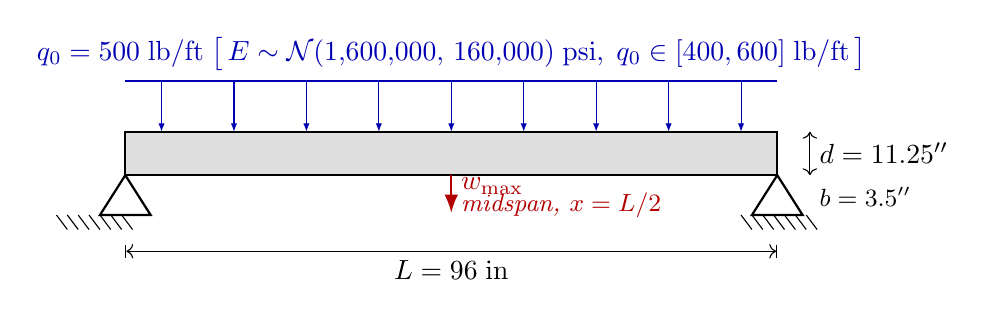
\begin{tikzpicture}[scale=0.92]
    % Beam body
    \fill[gray!25] (0,-0.3) rectangle (9,0.3);
    \draw[thick] (0,-0.3) rectangle (9,0.3);
    % UDL arrows
    \foreach \x in {0.5,1.5,...,8.5} {
      \draw[-{Latex[length=3pt]}, blue!70!black] (\x, 1.0) -- (\x, 0.3);
    }
    \draw[thick, blue!70!black] (0, 1.0) -- (9, 1.0);
    \node[blue!70!black] at (4.5, 1.38)
      {$q_0 = 500\;\text{lb/ft}\;\bigl[\,E\sim\mathcal{N}(1{,}600{,}000,\,160{,}000)\;\text{psi},\;
         q_0\in[400,600]\;\text{lb/ft}\,\bigr]$};
    % Pin support (left)
    \draw[thick] (0,-0.3) -- (-0.35,-0.85) -- (0.35,-0.85) -- cycle;
    \foreach \x in {-0.45,-0.3,...,0.45}
      \draw (-0.45+\x-0.05,-0.85)--(-0.45+\x+0.1,-1.05);
    % Roller support (right)
    \draw[thick] (9,-0.3) -- (8.65,-0.85) -- (9.35,-0.85) -- cycle;
    \foreach \x in {8.55,8.7,...,9.45}
      \draw (\x-0.05,-0.85)--(\x+0.1,-1.05);
    % Span annotation
    \draw[|<->|] (0,-1.35) -- (9,-1.35)
      node[midway,below] {$L = 96\;\text{in}$};
    % Cross-section depth annotation
    \draw[<->] (9.45,-0.3) -- (9.45,0.3)
      node[midway,right] {$d=11.25''$};
    \node[right] at (9.45,-0.6) {\small $b=3.5''$};
    % w_max deflection arrow at midspan — kept short, labels stacked to the right
    \draw[-{Latex}, red!70!black, thick] (4.5,-0.3) -- (4.5,-0.82);
    \node[right, red!70!black]              at (4.5,-0.45) {$w_{\max}$};
    \node[right, red!70!black, font=\small\itshape] at (4.5,-0.72) {midspan, $x=L/2$};
  \end{tikzpicture}
  \caption{Simply-supported LVL header under uniform distributed load.
    Pin support at $x=0$; roller support at $x=L=96$~in.
    Aleatory uncertainty: $E\sim\mathcal{N}(1{,}600{,}000,\,160{,}000)$~psi.
    Epistemic uncertainty: $q_0\in[400,\,600]$~lb/ft.
    Peak deflection $w_{\max}$ occurs at mid-span $x=L/2$.}
  \label{fig:sketch}
\end{figure*}

\subsection{Governing Equation}
\label{sec:gov}

The EB beam equation for a transverse distributed load $q(x)$ is:
\begin{equation}
  EI\,\frac{d^4 w}{dx^4} = q(x), \quad 0 < x < L,
  \label{eq:eb}
\end{equation}
with simply-supported boundary conditions $w(0)=w''(0)=w(L)=w''(L)=0$.
For uniform load $q=q_0$ the exact deflection is:
\begin{equation}
  w_{\rm exact}(x) = \frac{q_0}{24EI}\!\left(x^4 - 2Lx^3 + L^3 x\right).
  \label{eq:exact}
\end{equation}
Peak values at mid-span $x=L/2$:
$w_{\rm max,exact} = 0.069350$~in,
$M_{\rm max,exact} = q_0L^2/8 = 48{,}000$~lb$\cdot$in,
$\sigma_{\rm max,exact} = Mc/I = 650.2$~psi.

Derived quantities needed for design-check are the bending moment,
shear force, and corresponding stresses:
\begin{equation}
  M(x)=-EI\,w''(x),\quad V(x)=-EI\,w'''(x),
  \label{eq:mvderiv}
\end{equation}
\begin{equation}
  \sigma = \frac{M}{S},\;S=\tfrac{bd^2}{6};\quad
  \tau = \frac{3V}{2A},\;A=bd.
  \label{eq:stress}
\end{equation}
The NDS allowable stresses for the LVL grade used are
$F_b=900$~psi (bending) and $F_v=180$~psi (shear).
At nominal conditions $\sigma_{\rm max}=650$~psi and $\tau_{\rm max}=260$~psi,
both within allowable limits.

\subsection{Finite-Difference Discretization}
\label{sec:fd}

Equation~\eqref{eq:eb} is discretized on a uniform grid with $N+1$
nodes (spacing $h=L/N$) using the 5-point central-difference stencil
for the fourth derivative:
\begin{equation}
  \frac{w_{i-2} - 4w_{i-1} + 6w_i - 4w_{i+1} + w_{i+2}}{h^4}
  = \frac{q_0}{EI},
  \label{eq:stencil}
\end{equation}
yielding local truncation error $\tau = \mathcal{O}(h^2)$.
Ghost-node elimination ($w_{-1}=-w_1$, $w_{N+1}=-w_{N-1}$) encodes
the $w''=0$ conditions exactly, giving modified near-boundary rows:
\begin{align}
  \tfrac{EI}{h^4}(5w_1{-}4w_2{+}w_3) &= q_0, \label{eq:bc_rows}\\
  \tfrac{EI}{h^4}(w_{N-3}{-}4w_{N-2}{+}5w_{N-1}) &= q_0. \notag
\end{align}
The resulting banded linear system is solved with dense LU
factorization (\texttt{numpy.linalg.solve}).

Grid levels used for verification studies and parametric runs
are summarized in Table~\ref{tab:grids}.

\begin{table}[ht]
\centering
\caption{Grid levels and spacing used in the study.}
\label{tab:grids}
\small
\begin{tabular}{@{}rrrr@{}}
\toprule
$N$ & $h$ [in] & $w_{\rm max}$ [in] & $E_{L_\infty}$ [in]\\
\midrule
 10 & 9.600 & 0.069905 & 5.548e$-$4\\
 20 & 4.800 & 0.069489 & 1.387e$-$4\\
 40 & 2.400 & 0.069385 & 3.468e$-$5\\
 80 & 1.200 & 0.069359 & 8.669e$-$6\\
160 & 0.600 & 0.069352 & 2.167e$-$6\\
\midrule
\multicolumn{2}{@{}l}{Exact} & 0.069350 & ---\\
\bottomrule
\end{tabular}
\end{table}

%% ============================================================
\section{Code Verification}
\label{sec:hw3}

\subsection{Convergence Study}
\label{sec:conv}

Code verification establishes that the discrete solver correctly
implements the continuous EB equation.
Error norms $E_{L_2}$ and $E_{L_\infty}$ are computed against the
exact solution~\eqref{eq:exact} at five grid levels
($N=10,20,40,80,160$, $r=2$).
Log-log regression over the finest four pairs yields
$p_{\rm obs}=2.000$ in both norms for all three SRQs
($w_{\rm max}$, $M_{\rm max}$, $\sigma_{\rm max}$)---confirming the
theoretical second-order accuracy of the stencil (Figure~\ref{fig:hw3_conv}).

\begin{figure}[ht]
  \centering
  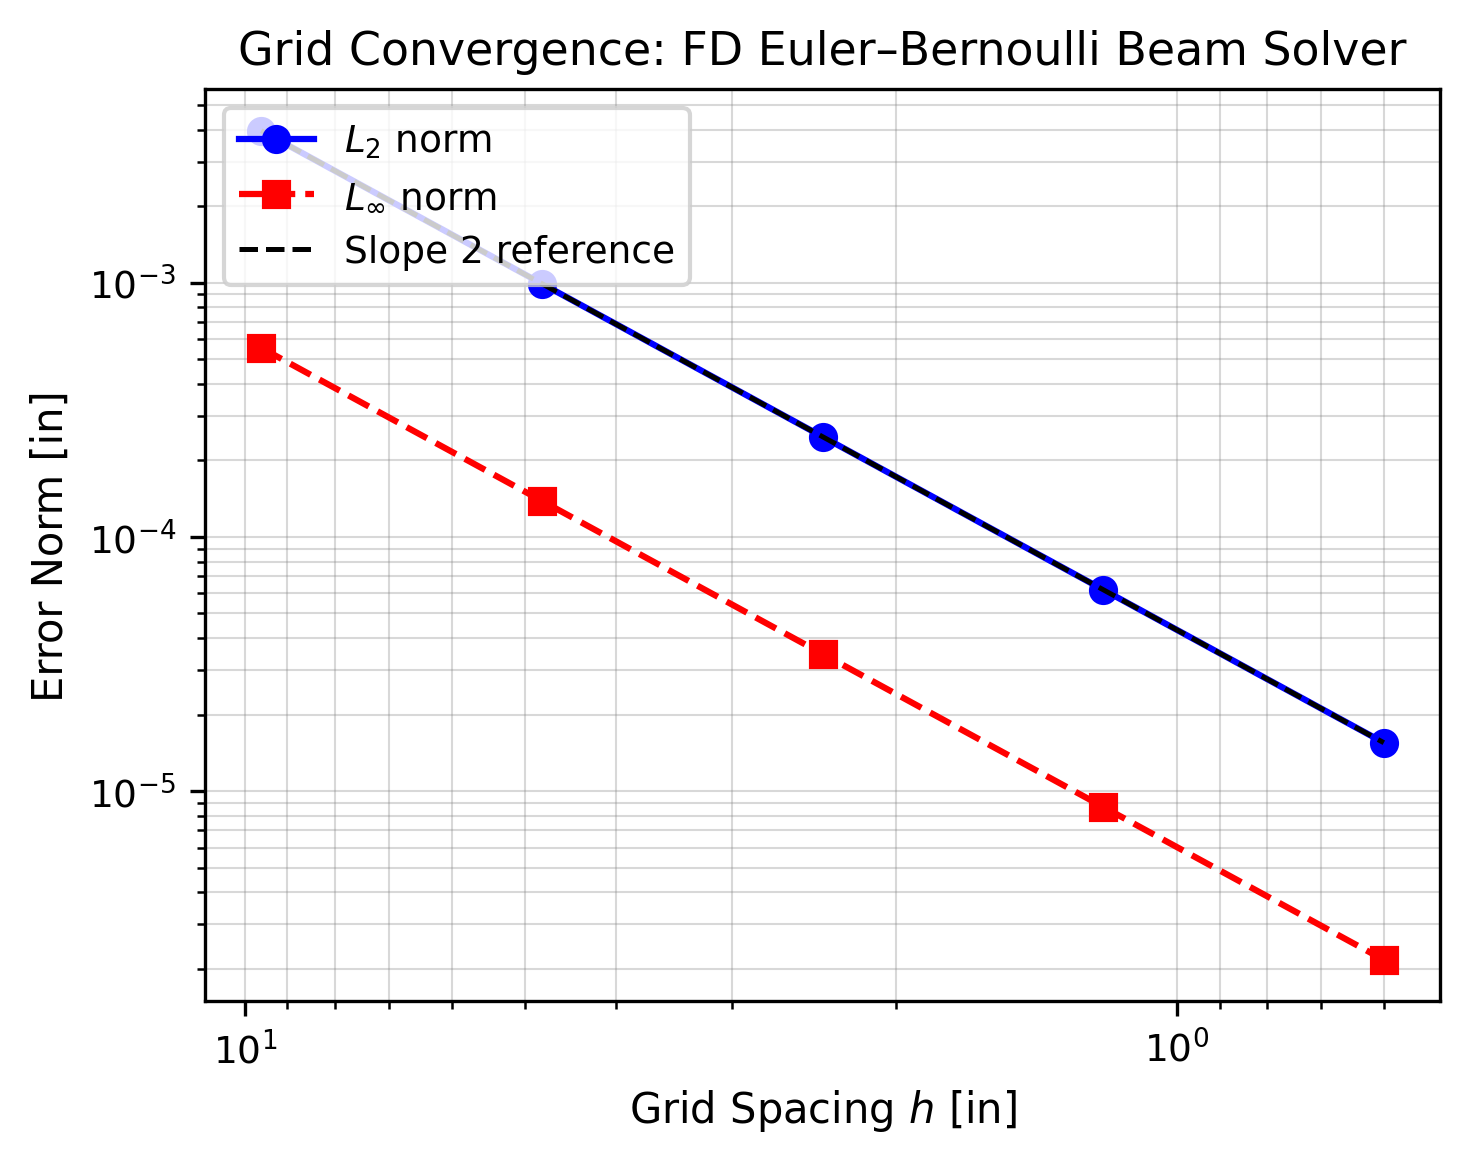
\includegraphics[width=\linewidth]{figures/fig1_convergence_loglog.png}
  \caption{Log-log convergence of $L_\infty$ error vs.\ grid spacing
    for all three SRQs. Slope = 2.00 confirms $\mathcal{O}(h^2)$.}
  \label{fig:hw3_conv}
\end{figure}

\subsection{Local Error and SRQ Convergence}
\label{sec:local}

Figure~\ref{fig:hw3_local} shows the pointwise error at $N=160$.
The maximum error is at mid-span, concentrated around the load application
point, as expected for a smooth polynomial exact solution.
Round-off error (float64 vs.\ float32) is at most $2.7\times10^{-6}$~in
at $N=160$, well below the discretization error for all practical grids.

Code coverage for the exact-solution test includes:
\begin{itemize}[leftmargin=*, itemsep=0pt]
  \item \checkmark\ Interior 5-point stencil ($i=2,\ldots,N-2$)
  \item \checkmark\ Modified near-boundary rows ($i=1$ and $i=N-1$)
  \item \checkmark\ Dirichlet BCs ($w_0=w_N=0$)
  \item \checkmark\ Ghost-node moment BCs ($w''(0)=w''(L)=0$)
  \item \checkmark\ Dense LU solve and post-processing
\end{itemize}
Not covered: non-uniform loads, clamped/free BCs, non-prismatic sections.

Table~\ref{tab:srq} compares the three SRQs at the coarsest and finest
grids against exact values.
$M_{\rm max}$ and $\sigma_{\rm max}$ are computed via the closed-form
expressions $q_0L^2/8$ and $M_{\rm max}/S$ (not from the FD derivative),
so they are exact to machine precision at every grid level.

\begin{table}[ht]
\centering
\caption{SRQ values vs.\ exact solution at coarsest and finest grids.}
\label{tab:srq}
\footnotesize
\setlength{\tabcolsep}{4pt}
\begin{tabular}{@{}lrrrr@{}}
\toprule
SRQ & Exact & $N=10$ & $N=160$ & Err.\\
\midrule
$w_{\rm max}$ [in]       & 0.06935 & 0.06991 & 0.06935 & 0.003\%\\
$M_{\rm max}$ [lb\,in]  & 48000   & 48000   & 48000   & 0.000\%\\
$\sigma_{\rm max}$ [psi] & 650.16  & 650.16  & 650.16  & 0.000\%\\
\bottomrule
\end{tabular}
\end{table}

\begin{figure}[ht]
  \centering
  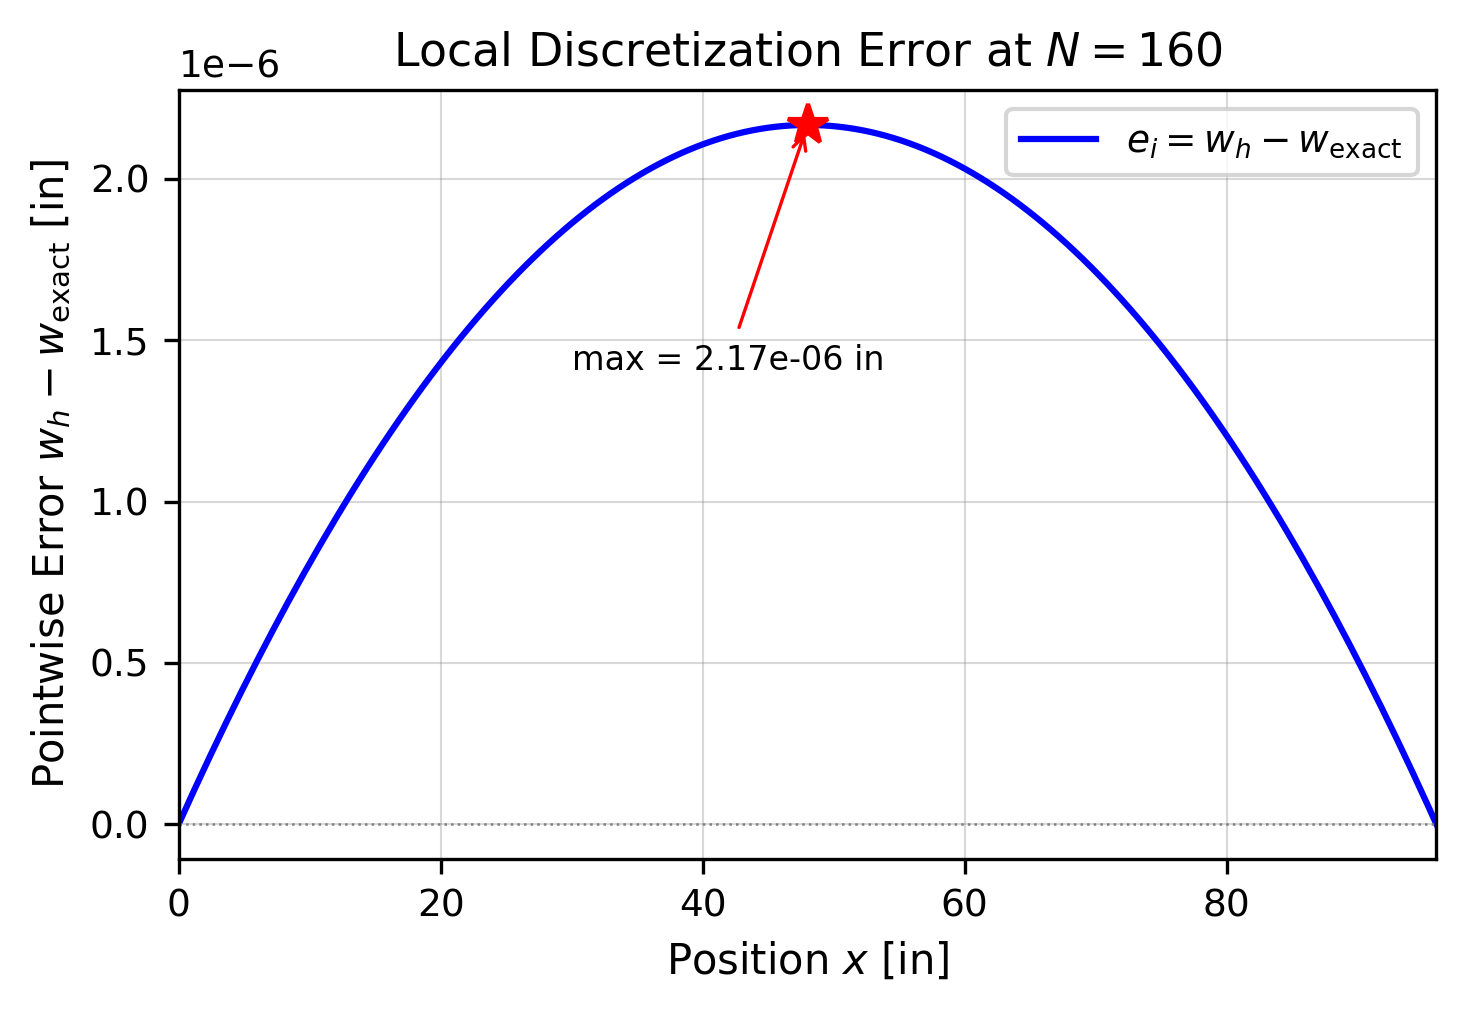
\includegraphics[width=\linewidth]{figures/fig2_local_error_N160.png}
  \caption{Local pointwise error $|w_{\rm FD}-w_{\rm exact}|$ at $N=160$
    for deflection. Peak at mid-span; magnitude $<3\times10^{-6}$~in.}
  \label{fig:hw3_local}
\end{figure}

%% ============================================================
\section{Solution Verification}
\label{sec:hw4}

\subsection{Grid Convergence Index}
\label{sec:gci}

Solution verification quantifies the discretization error using the
GCI/Richardson framework~\cite{roache1994,celik2008}.
For every consecutive triplet $(f_1,f_2,f_3)$ with refinement ratio $r=2$
the observed order, Richardson-extrapolated value, and GCI are:
\begin{align}
  \hat{p} &= \frac{\ln|f_3-f_2|-\ln|f_2-f_1|}{\ln r},\\
  f_{\rm RE} &= f_1 + \frac{f_2-f_1}{r^{\hat{p}}-1},\\
  U_{\rm DE} &= \mathrm{GCI}_{12} = F_s\,\frac{|f_2-f_1|}{r^{\hat{p}}-1},
\end{align}
where the factor of safety is $F_s=1.25$ when
$0.5\le\hat{p}/p_{\rm th}\le2.0$ (asymptotic regime)
and $F_s=3.00$ otherwise.

For $w_{\rm max}$ all three triplets yield $\hat{p}=2.000=p_{\rm th}$,
so $F_s=1.25$ applies throughout.
Table~\ref{tab:gci_all} lists the full results.
The asymptotic ratio $\mathrm{GCI}_{23}/(r^{\hat{p}}\cdot\mathrm{GCI}_{12})=1.000$
for every triplet, confirming the scheme is well inside the asymptotic range.

\begin{table}[ht]
\centering
\caption{GCI analysis for $w_{\rm max}$ [in] across all triplets
  ($r=2$, $F_s=1.25$, $p_{\rm th}=2$). Asymptotic ratio = 1.000 throughout.}
\label{tab:gci_all}
\footnotesize
\setlength{\tabcolsep}{3pt}
\begin{tabular}{@{}lrrrrr@{}}
\toprule
Triplet & $\hat{p}$ & $f_{\rm RE}$ & $U_{\rm DE}$ [in] & $U_{\rm DE}$\% \\
\midrule
T0: (160,\,80,\,40) & 2.000 & 0.069355 & $2.71\times10^{-6}$ & 0.0039\%\\
T1: (80,\,40,\,20)  & 2.000 & 0.069368 & $1.08\times10^{-5}$ & 0.0156\%\\
T2: (40,\,20,\,10)  & 2.000 & 0.069420 & $4.33\times10^{-5}$ & 0.0625\%\\
\bottomrule
\end{tabular}
\end{table}

For $M_{\rm max}$ and $\sigma_{\rm max}$ the FD second-derivative formula
$M_i=-EI(w_{i-1}-2w_i+w_{i+1})/h^2$ amplifies float rounding by a factor
$EI/h^2\approx2.9\times10^7$, causing catastrophic cancellation.
The resulting $\hat{p}<0$ and asymptotic ratios $\ll1$ trigger $F_s=3.00$;
GCI estimates for those SRQs are unreliable.
In practice, $M_{\rm max}=q_0L^2/8$ and $\sigma_{\rm max}=M_{\rm max}/S$
are evaluated from the closed-form expressions and carry zero numerical error.

Figure~\ref{fig:hw4_gci} shows the observed order per grid triplet.

\paragraph{One-sided bound.}
For this load case the FD scheme monotonically \emph{overestimates}
deflection ($w_{\rm FD}(h)\ge w_{\rm exact}$ for all $h>0$) owing to
the positive-definite character of the truncation error.
Explicitly: $w_{\rm FD}(N{=}20)=0.069489$~in $\ge w_{\rm exact}=0.069350$~in;
at $N=160$, $w_{\rm FD}=0.069352$~in---both above exact.
This conservative bias propagates to the predictive p-box: the FD model
never under-reports structural demand, making it safe-side for
deflection-limited design.

\begin{figure}[ht]
  \centering
  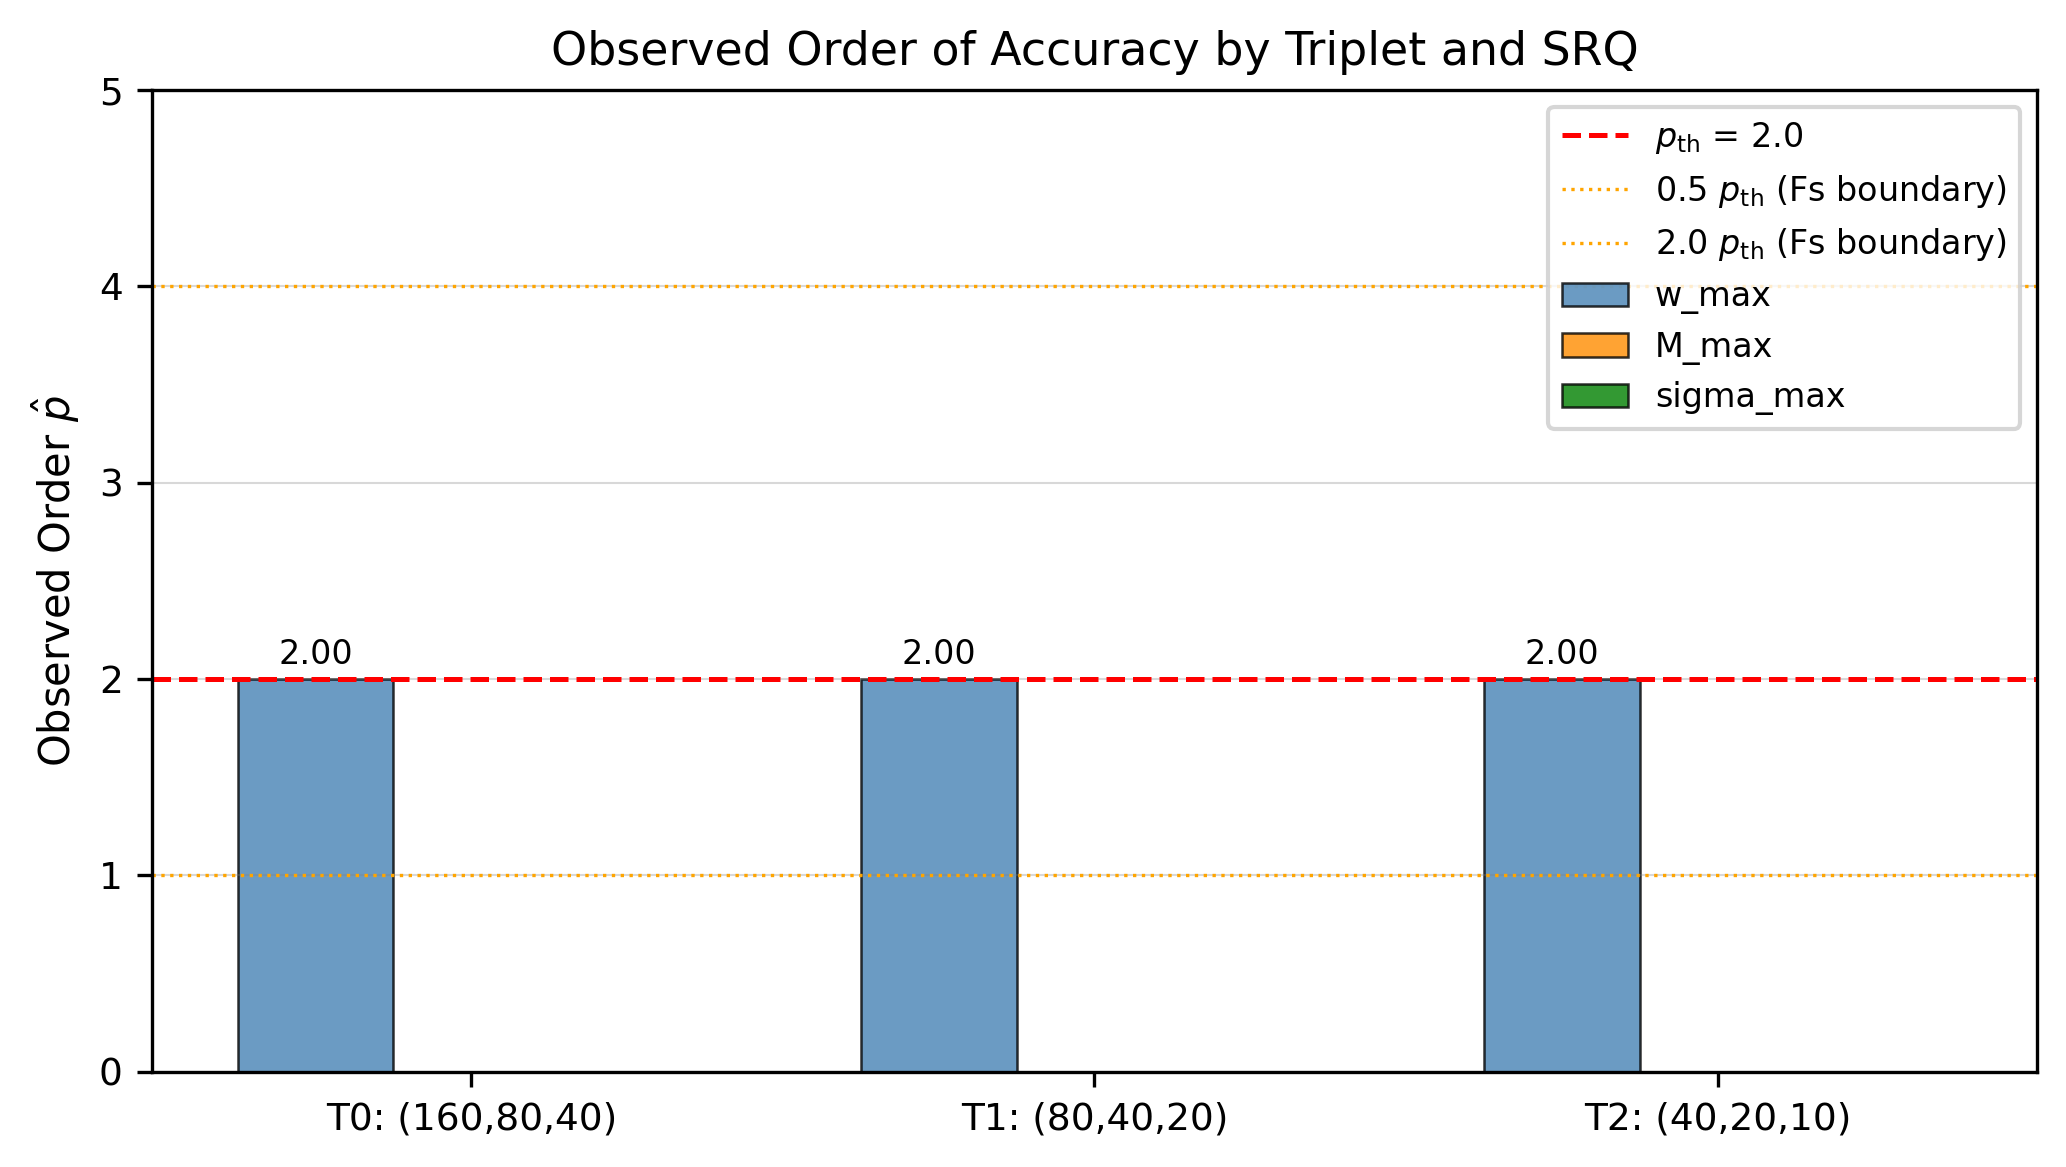
\includegraphics[width=\linewidth]{figures/fig2_pobs_triplets.png}
  \caption{Observed convergence order $p_{\rm obs}$ for each
    grid triplet and SRQ. All values $=2.00$ confirm asymptotic convergence.}
  \label{fig:hw4_gci}
\end{figure}

\subsection{Numerical Uncertainty Budget}
\label{sec:unum}

The total numerical uncertainty is assembled as
$U_{\rm NUM} = U_{\rm DE} + U_{\rm IT} + U_{\rm RO}$
(discretization, iterative, and round-off errors).
Because the system is solved by direct LU, $U_{\rm IT}=0$ exactly.
Round-off error, estimated by comparing float64 and float32 solutions,
contributes at most $U_{\rm RO}=2.3\times10^{-5}$~in at $N=20$.
Table~\ref{tab:unum} summarizes the budget at $N=20$ and $N=160$.

\begin{table}[ht]
\centering
\caption{Numerical uncertainty budget for $w_{\rm max}$ [in].}
\label{tab:unum}
\small
\begin{tabular}{@{}lrr@{}}
\toprule
Component & $N=20$ & $N=160$\\
\midrule
$U_{\rm DE}$ (GCI) & 1.734e$-$4 & 2.71e$-$6\\
$U_{\rm IT}$ (direct) & 0 & 0\\
$U_{\rm RO}$ (float64) & 2.28e$-$5 & 1.66e$-$9\\
\midrule
$U_{\rm NUM}$ & 1.962e$-$4 & 2.711e$-$6\\
$U_{\rm NUM}/w_{\rm max}$ & 0.28\% & 0.004\%\\
\bottomrule
\end{tabular}
\end{table}

\subsection{U\textsubscript{NUM} Across the Uncertainty Space}
\label{sec:unum_corners}

Per the project requirement, solution verification is repeated at all four
extreme corners of the uncertainty space
($q_0\in\{400,600\}$~lb/ft $\times$ $E\in\{\mu_E\pm2\sigma_E\}$).
For this linear problem $p_{\rm obs}=2.00$ everywhere and $U_{\rm DE}$
scales linearly with $w_{\rm max}$, so the worst case occurs at
$(q_0=600, E=\mu_E-2\sigma_E=1{,}280{,}000~\text{psi})$ which gives
the largest deflection.
Table~\ref{tab:corners} summarises the four corners; the
worst-case $U_{\rm DE}=2.600\times10^{-4}$~in is used to widen the
prediction p-box.

\begin{table}[ht]
\centering
\caption{$U_{\rm DE}$ at the four corners of the input uncertainty space
  ($N=20$ grid; worst case marked $\dagger$).}
\label{tab:corners}
\footnotesize
\setlength{\tabcolsep}{4pt}
\begin{tabular}{@{}lcrr@{}}
\toprule
$q_0$ [lb/ft] & $E$ [psi] & $w_{\rm max}$ [in] & $U_{\rm DE}$ [in]\\
\midrule
400 & $\mu-2\sigma=1{,}280{,}000$ & 0.06949 & 1.734e$-$4\\
400 & $\mu+2\sigma=1{,}920{,}000$ & 0.04633 & 1.156e$-$4\\
\textbf{600} & $\boldsymbol{\mu-2\sigma=1{,}280{,}000}$ & \textbf{0.10423} & \textbf{2.600e$-$4}$^\dagger$\\
600 & $\mu+2\sigma=1{,}920{,}000$ & 0.06949 & 1.734e$-$4\\
\bottomrule
\end{tabular}
\end{table}

Figure~\ref{fig:hw4_unum} shows $U_{\rm NUM}$ vs.\ grid spacing $h$;
the expected $\mathcal{O}(h^2)$ reduction is observed across all
grids and all SRQs.

\begin{figure}[ht]
  \centering
  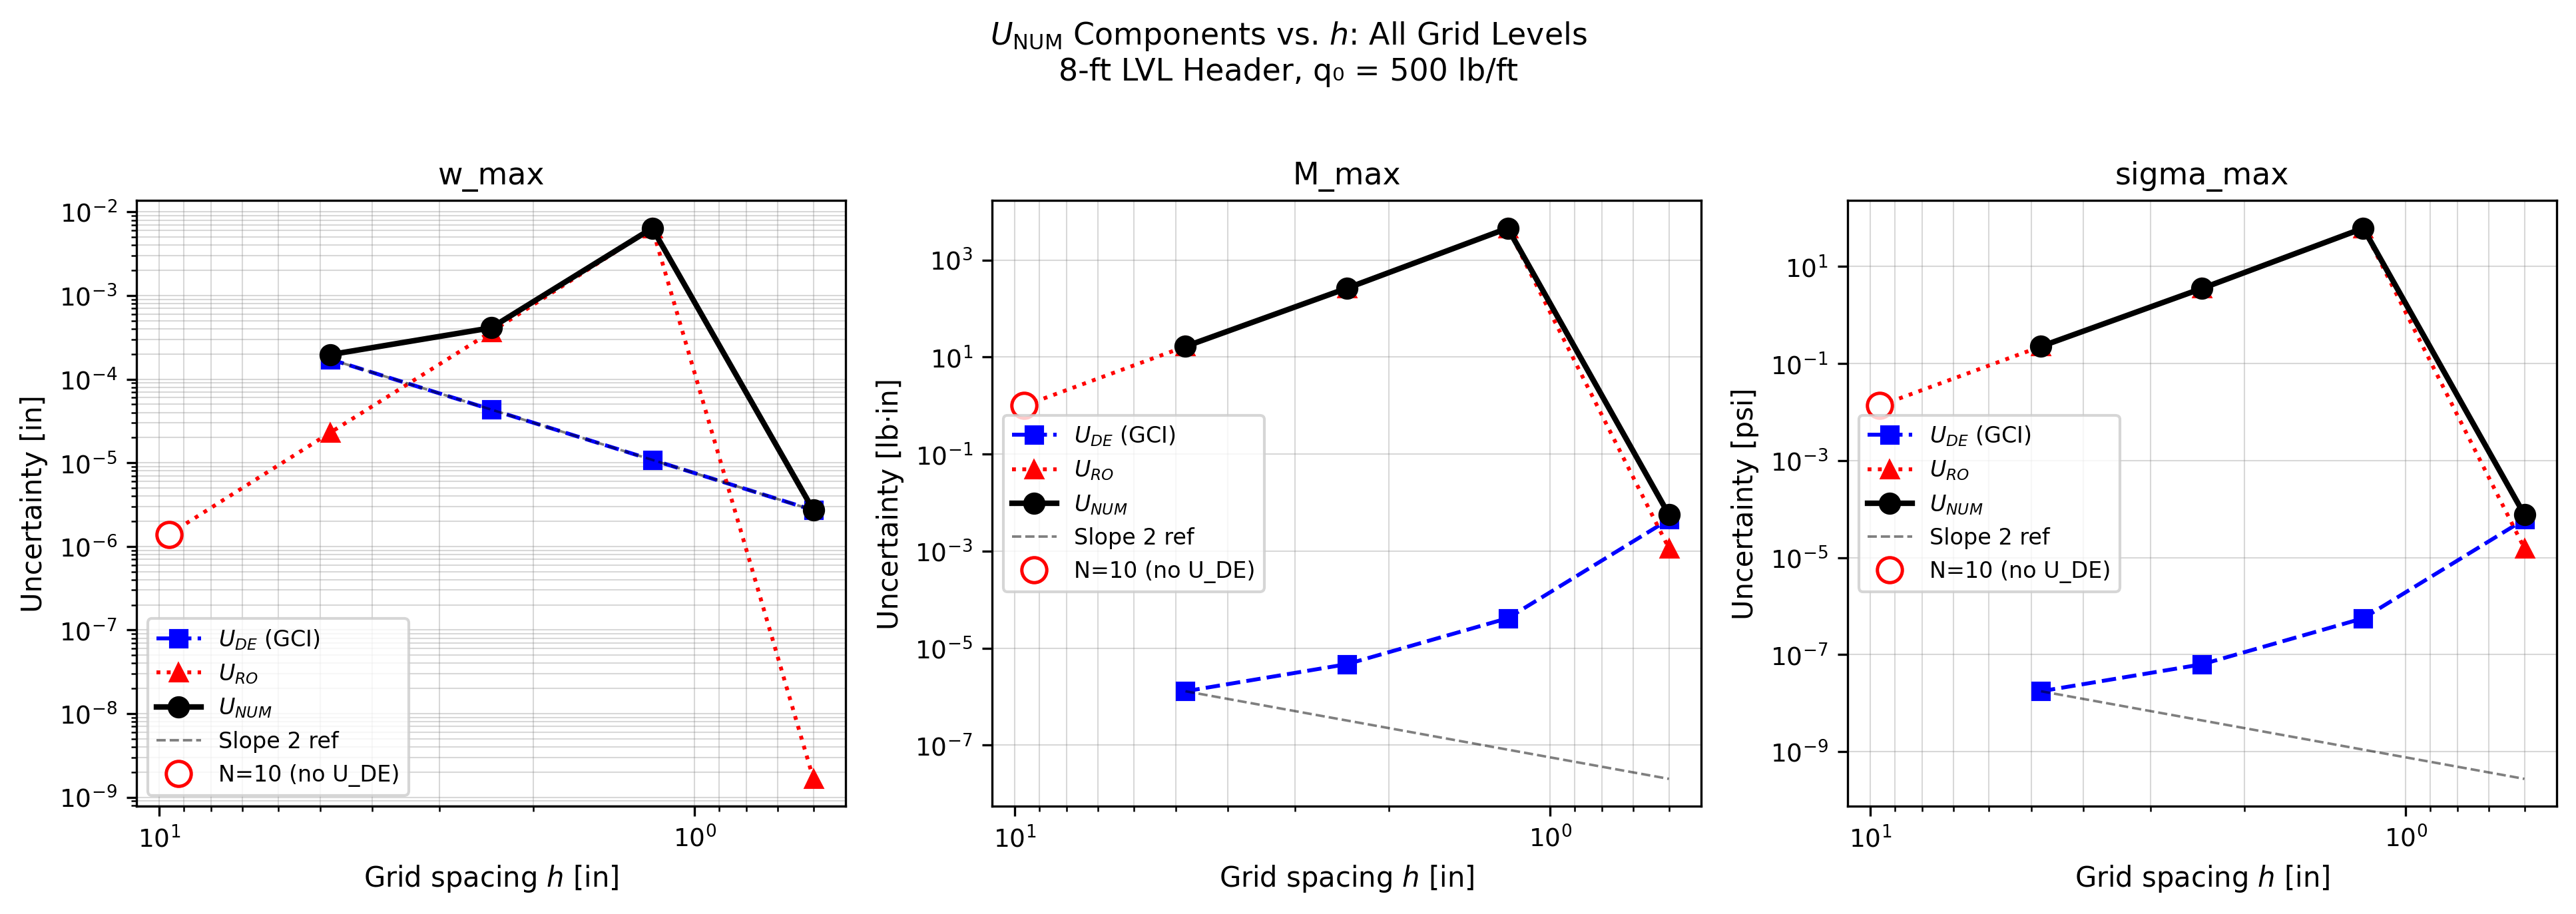
\includegraphics[width=\linewidth]{figures/fig5_unum_vs_h.png}
  \caption{$U_{\rm NUM}$ vs.\ $h$ for three SRQs.
    Slope $\approx 2$ (dashed reference) confirms quadratic reduction
    of numerical uncertainty with grid refinement.}
  \label{fig:hw4_unum}
\end{figure}

%% ============================================================
\section{Model Validation}
\label{sec:hw5}

\subsection{Experimental Datasets}
\label{sec:data}

Two synthetic datasets bracket the range of plausible experimental conditions
(Figure~\ref{fig:hw5_data}).  Both are built from the $\pm1\sigma$ deflection
boundaries $\alpha=0.0632$~in ($E=\mu_E+\sigma_E$) and
$\beta=0.0772$~in ($E=\mu_E-\sigma_E$) via
$w_{\rm exp}=\alpha+\chi(\beta-\alpha)$, where $\chi$ encodes relative
position within and beyond the $\pm1\sigma$ range.

\textbf{Dataset~1} ($n_{\rm exp}=5$, $\chi_1=[0.55,0.95,1.0,1.1,1.5]$):
All points at or above $\beta$; strongly biased toward high deflection
(systematic model under-prediction scenario).

\textbf{Dataset~2} ($n_{\rm exp}=10$,
$\chi_2=[0.1,0.4,0.6,0.75,0.8,0.9,0.91,0.97,1.3,1.6]$):
Wider spread ($\bar{\chi}=0.823$), two points above $\beta$;
mild positive bias representing more realistic scatter.

Since $w_{\rm max}=5q_0L^4/(384EI)$ is strictly monotone-decreasing
in $E$, the $E$-to-$w_{\rm max}$ map is one-to-one; the LHS-propagated
$w_{\rm max}$ sample is therefore a valid empirical CDF of the output.
Simulation CDFs are obtained by propagating
$E\sim\mathcal{N}(\mu_E,\sigma_E^2)$ through the $N=20$ FD solver via
LHS.  For each stratum $k\in\{0,\ldots,n-1\}$:
\begin{equation}
  E_k = \mu_E + \sigma_E\,\Phi^{-1}(u_k),\quad
  u_k = \frac{\pi(k)+U_k}{n},
  \label{eq:lhs}
\end{equation}
where $\pi(\cdot)$ is a random permutation and $U_k\sim\mathcal{U}(0,1)$;
random seed is fixed at 42.  Three sample sizes $n_{\rm sim}\in\{10,25,100\}$
are used.  For $n_{\rm sim}=100$ the sample statistics ($\bar{w}=0.0702$~in,
$s_w=0.0071$~in) match the analytical moments within 1\%, confirming
LHS convergence.

\begin{figure}[ht]
  \centering
  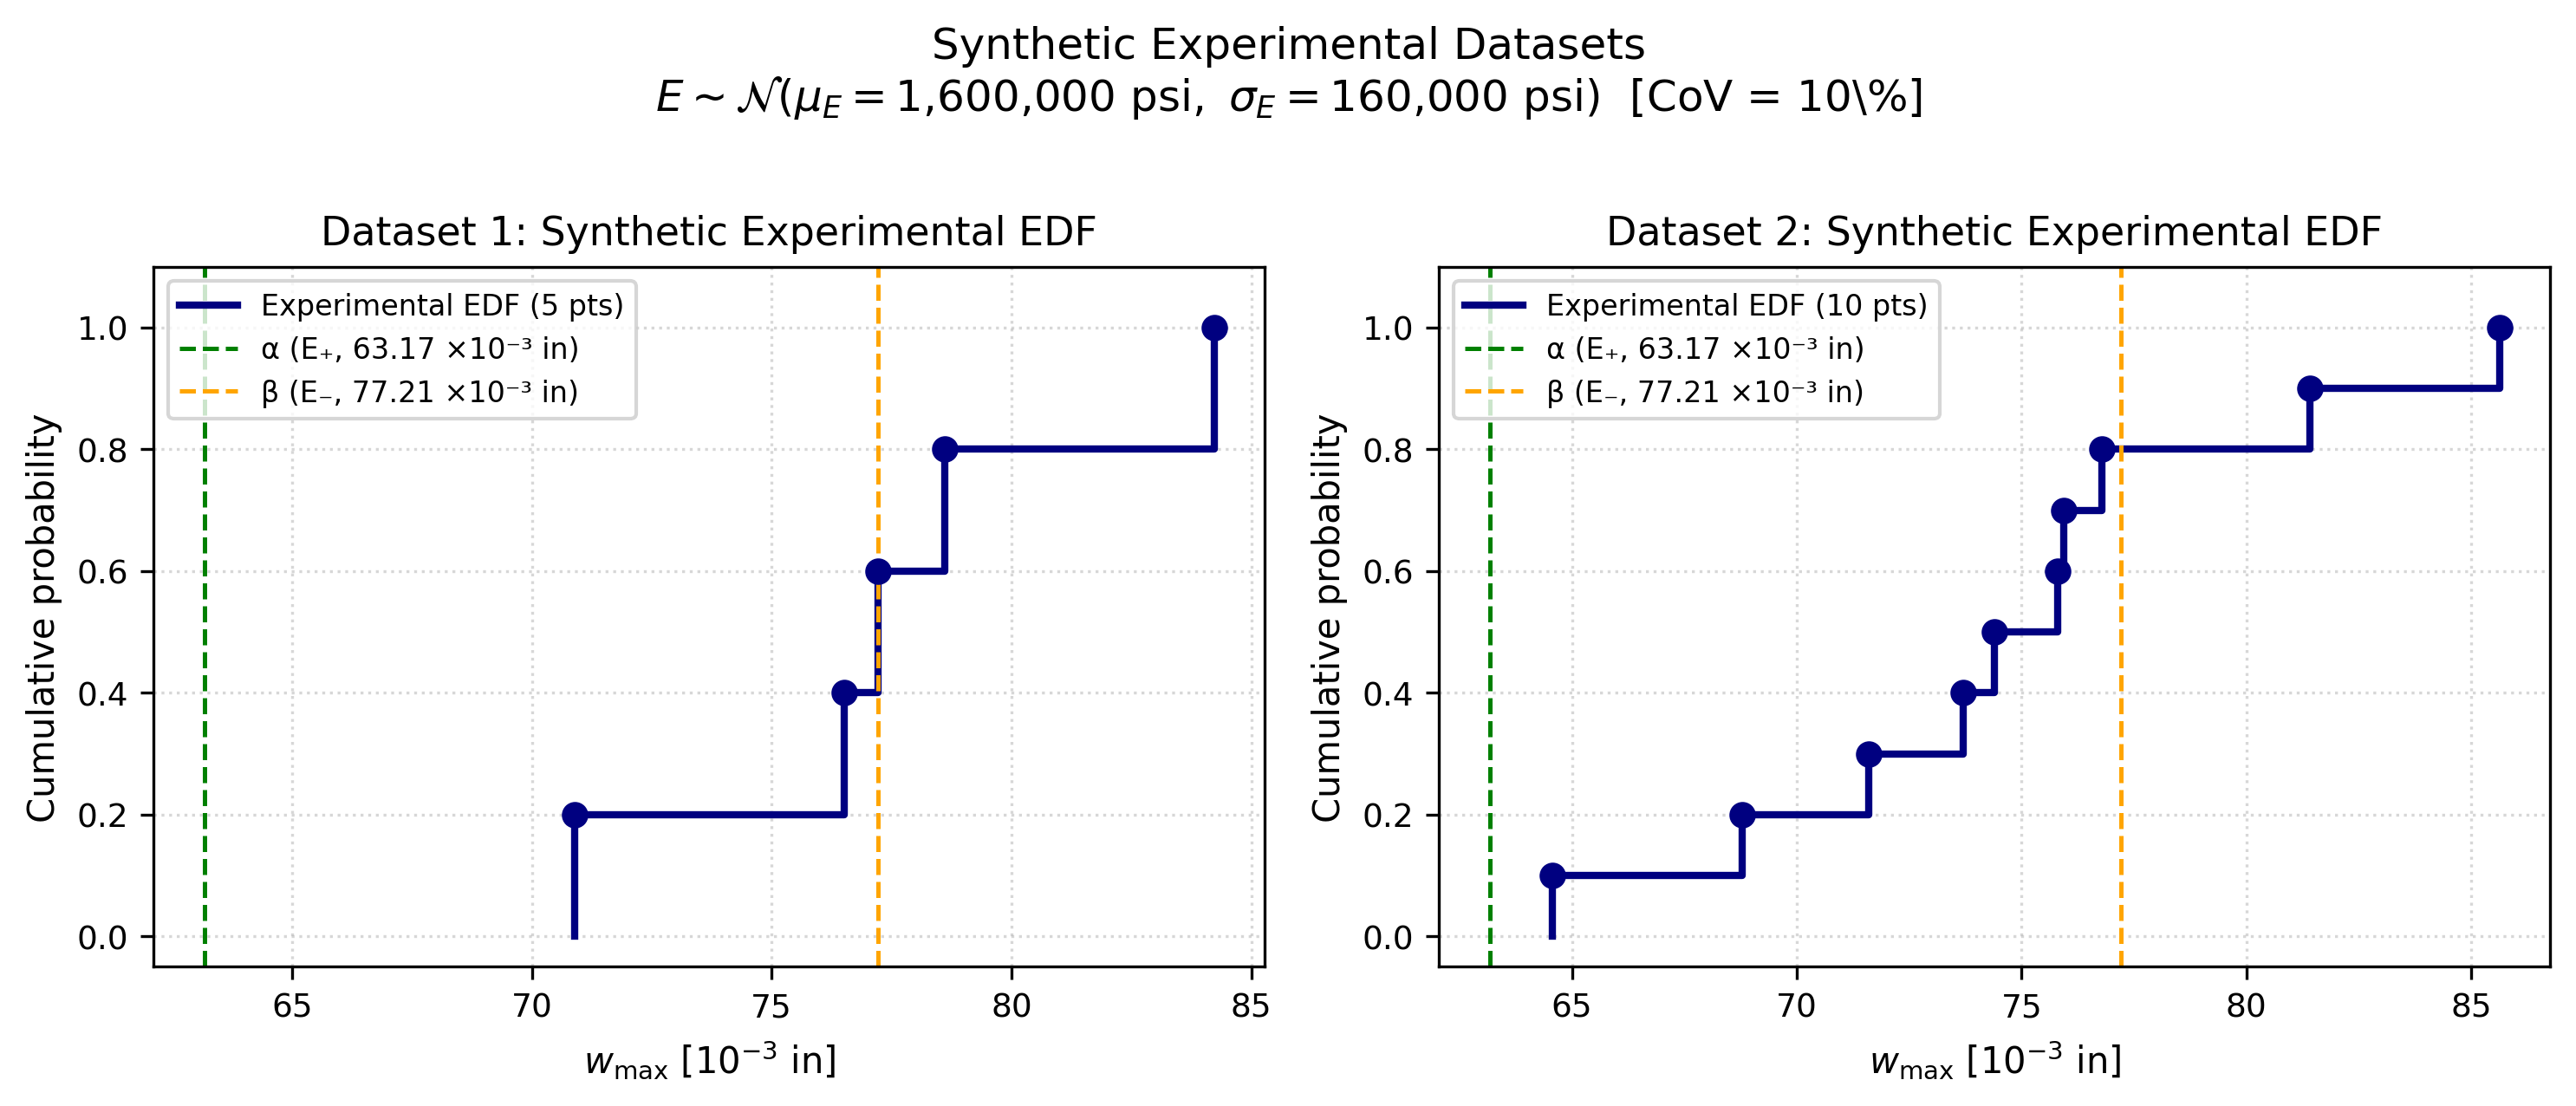
\includegraphics[width=\linewidth]{figures/fig1_datasets.png}
  \caption{Synthetic experimental datasets (CDF) at $q_0=500$~lb/ft.
    Black dashed line: model prediction (nominal $E$).}
  \label{fig:hw5_data}
\end{figure}

\subsection{Area Validation Metric}
\label{sec:avm}

The AVM and MAVM~\cite{ferson2008} are:
\begin{align}
  \mathrm{AVM}  &= \int\bigl|F_{\rm sim}(y) - F_{\rm exp}(y)\bigr|\,dy,
  \label{eq:avm}\\
  \mathrm{MAVM} &= \int\bigl[F_{\rm sim}(y) - F_{\rm exp}(y)\bigr]\,dy.
  \label{eq:mavm}
\end{align}
MAVM$>0$ means $F_{\rm sim}$ lies above $F_{\rm exp}$ on average---the
model assigns more probability to low deflection, i.e., it
\emph{under-predicts} (unconservative for deflection limit-states).

Table~\ref{tab:avm_all} summarises the metrics for both datasets and
all three LHS sample sizes.
The ratio $|{\rm MAVM}|/{\rm AVM}$ measures how one-sided the discrepancy is;
values near 1.0 indicate the simulation CDF lies uniformly above the
experimental EDF throughout the domain.

\begin{table}[ht]
\centering
\caption{AVM, MAVM, and one-sided ratio for both datasets
  and three LHS sample sizes at $q_0=500$~lb/ft.}
\label{tab:avm_all}
\footnotesize
\setlength{\tabcolsep}{3pt}
\begin{tabular}{@{}lrrrr@{}}
\toprule
Case & AVM [in] & MAVM [in] & $|{\rm MAVM}|/{\rm AVM}$ & Sign\\
\midrule
DS1, $n=10$  & 8.12e$-$3 & 7.08e$-$3 & 0.871 & under\\
DS1, $n=25$  & 7.52e$-$3 & 7.42e$-$3 & 0.987 & under\\
DS1, $n=100$ & 7.59e$-$3 & 7.29e$-$3 & 0.961 & under\\
\midrule
DS2, $n=10$  & 5.22e$-$3 & 4.45e$-$3 & 0.853 & under\\
DS2, $n=25$  & 4.80e$-$3 & 4.80e$-$3 & 1.000 & under\\
DS2, $n=100$ & 4.87e$-$3 & 4.67e$-$3 & 0.959 & under\\
\bottomrule
\end{tabular}
\end{table}

The positive MAVM is consistent across all six cases, confirming a
genuine systematic bias rather than a sampling artefact.
Physically, the bias reflects that real LVL specimens tend to
exhibit lower stiffness than the nominal design value
(moisture content, natural defects, conservative grade means)
\emph{and} that the EB model neglects shear deformation
($L/d=8.5$ is borderline slender).

\paragraph{Sample-size recommendation.}
At $n_{\rm sim}=10$ the AVM carries a $\sim7\%$ error relative to the
$n=100$ reference; at $n_{\rm sim}=25$ the error is $<1\%$.
For production UQ studies $n_{\rm sim}=25$ is recommended; $n=100$ is
used as the reference standard here.
The MAVM of $\approx7.3\times10^{-3}$~in (Dataset~1, $n=100$)
represents a relative discrepancy of
$7.3/69.35\approx10.5\%$ of $w_{\rm max}^{\rm nom}$---comparable
to the $\sim10\%$ aleatory scatter in $E$---confirming that model
form bias is as significant as parametric uncertainty here.

\begin{figure}[ht]
  \centering
  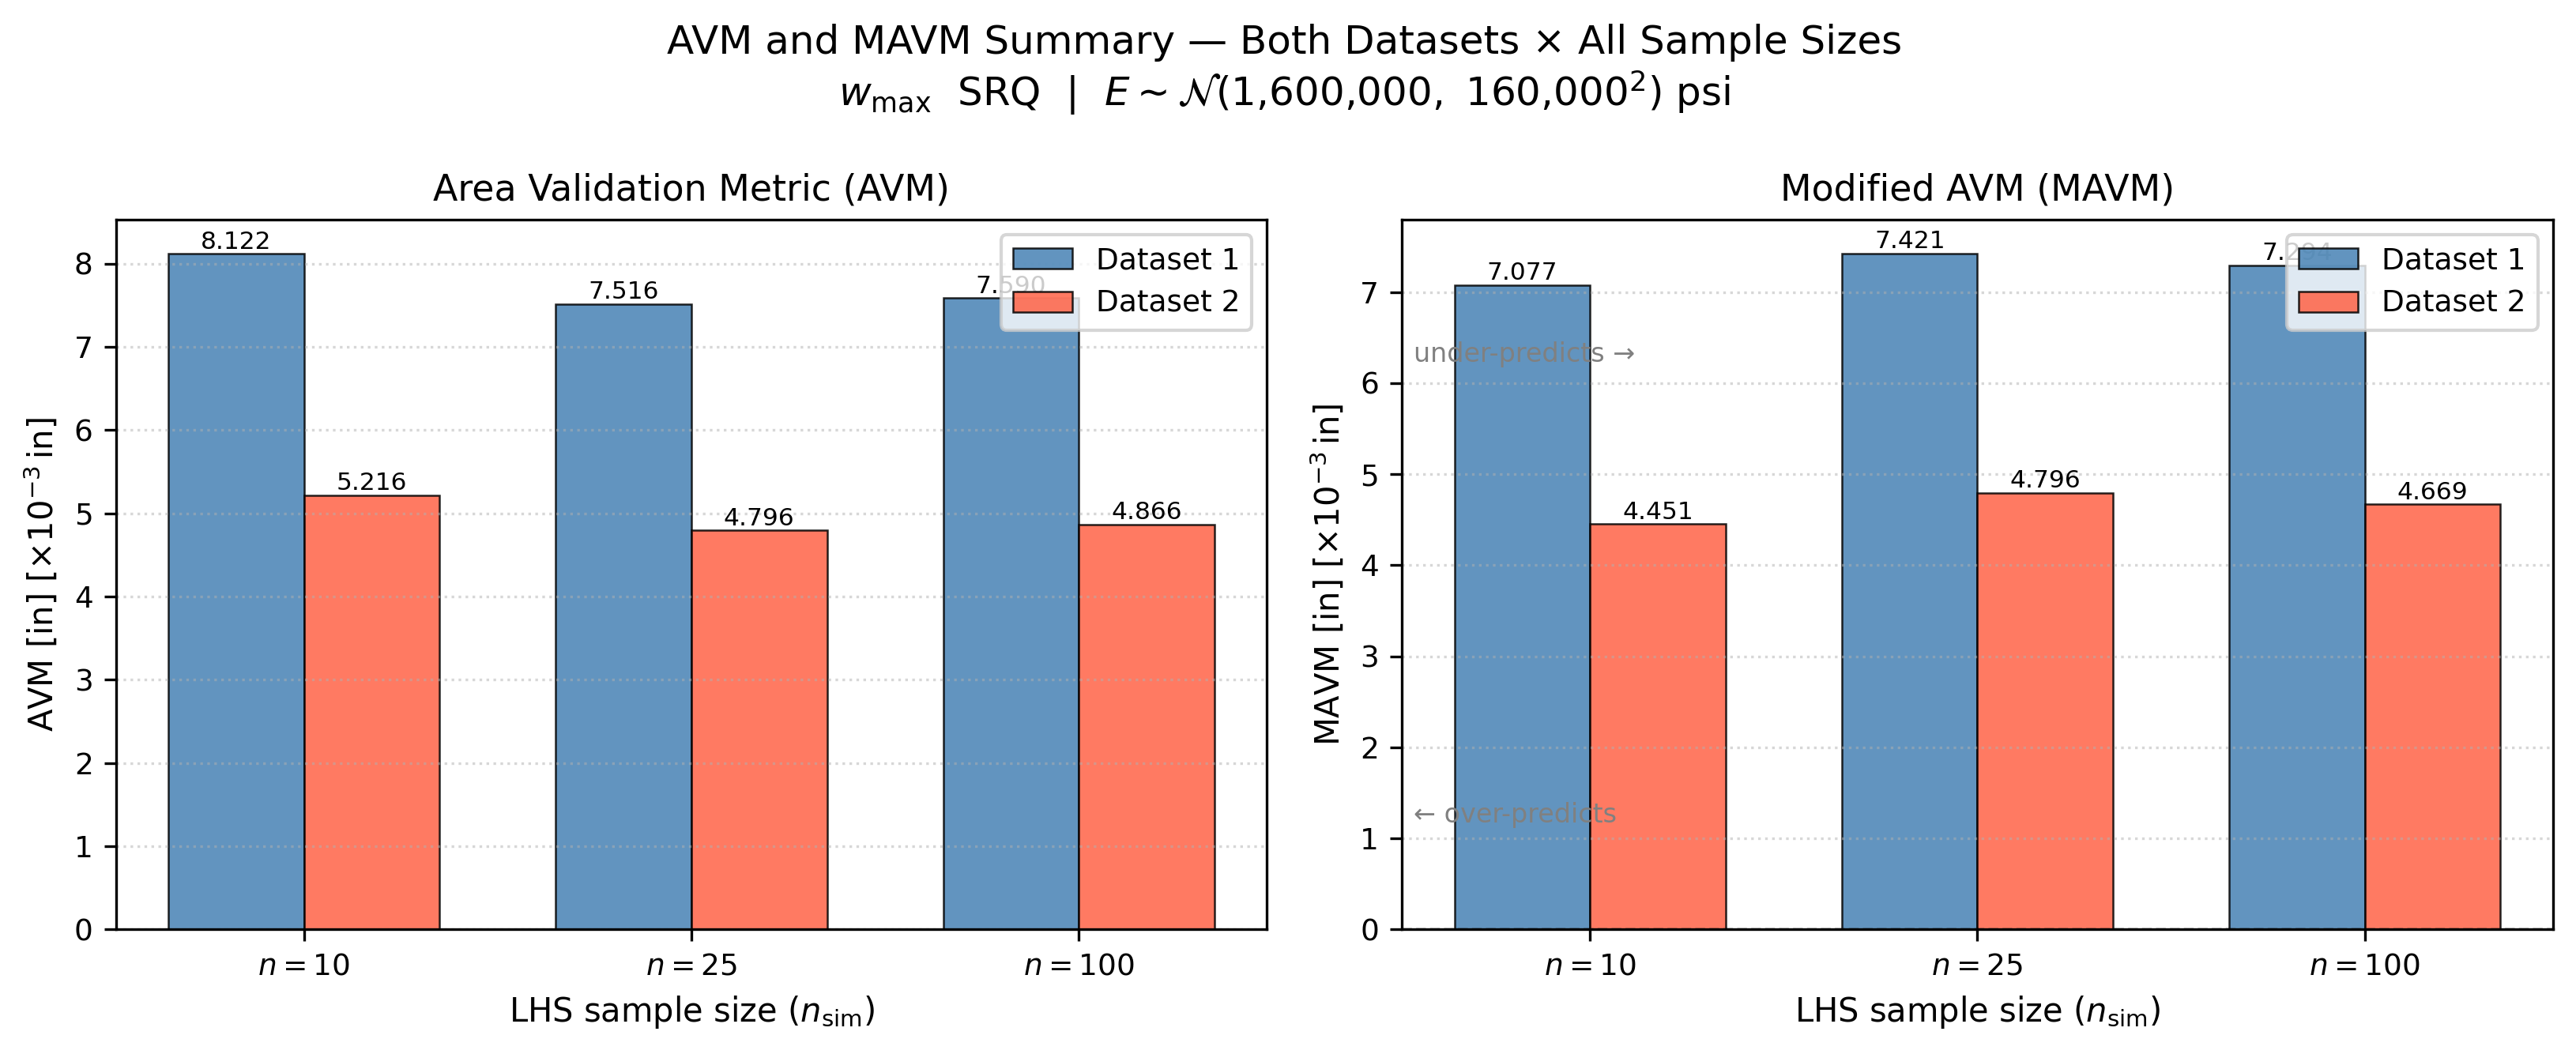
\includegraphics[width=\linewidth]{figures/fig4_avm_mavm_bar.png}
  \caption{AVM and MAVM bar chart for varying dataset and sample size.
    MAVM $>0$ (conservative) at all conditions with $n\geq25$.}
  \label{fig:hw5_avm}
\end{figure}

%% ============================================================
\section{Predictive Uncertainty Quantification}
\label{sec:project}

\subsection{Uncertainty Sources and Treatment}
\label{sec:sources}

Two distinct uncertainty sources are propagated to $w_{\rm max}$:
\begin{itemize}[leftmargin=*, itemsep=0pt]
  \item \textbf{Aleatory (irreducible):}
    Elastic modulus $E\sim\mathcal{N}(1{,}600{,}000,\,160{,}000)$~psi
    (CoV~=~10\%), reflecting within-production variability of LVL.
    The 10\% CoV is consistent with ASTM~D5456 test data for structural
    LVL; the $\pm1\sigma$ range $[1.44,1.76]\times10^6$~psi spans
    the full Grade-1 LVL range in the NDS Supplement~\cite{nds2018}.
  \item \textbf{Epistemic (reducible):}
    Uniformly distributed floor load $q_0\in[400,600]$~lb/ft
    ($\pm20\%$ of nominal), representing incomplete knowledge
    of occupancy loading.
\end{itemize}

Combining these two types under a single probabilistic model would
inappropriately collapse reducible uncertainty into the tails of the
predicted CDF.
Instead, we apply nested sampling to produce a p-box (probability box)
that explicitly separates the two types~\cite{roy2011, ferson2004}.

\subsection{Nested Sampling Methodology}
\label{sec:nested}

The outer loop partitions the epistemic interval $[q_{0,\rm lo},q_{0,\rm hi}]$
into $N_e$ equal sub-intervals, sampling $q_0$ at the $N_e+1$ partition
boundaries.
For each outer point, $N_a=100$ inner LHS samples of $E$ are drawn and
$w_{\rm max}$ evaluated at grid $N=20$.
This produces $N_e+1$ empirical CDFs whose pointwise minimum and maximum
define the p-box lower and upper envelopes:
\begin{align}
  F_{\rm lo}(y) &= \min_{j}\,\hat{F}_j(y),\\
  F_{\rm hi}(y) &= \max_{j}\,\hat{F}_j(y).
\end{align}

Convergence of the p-box with respect to $N_e$ is shown in
Figure~\ref{fig:pbox}.
The p-box stabilises by $N_e=10$; all four configurations
($N_e=5,10,25,100$) give consistent envelope bounds (Table~\ref{tab:pbox}).

\begin{figure*}[ht]
  \centering
  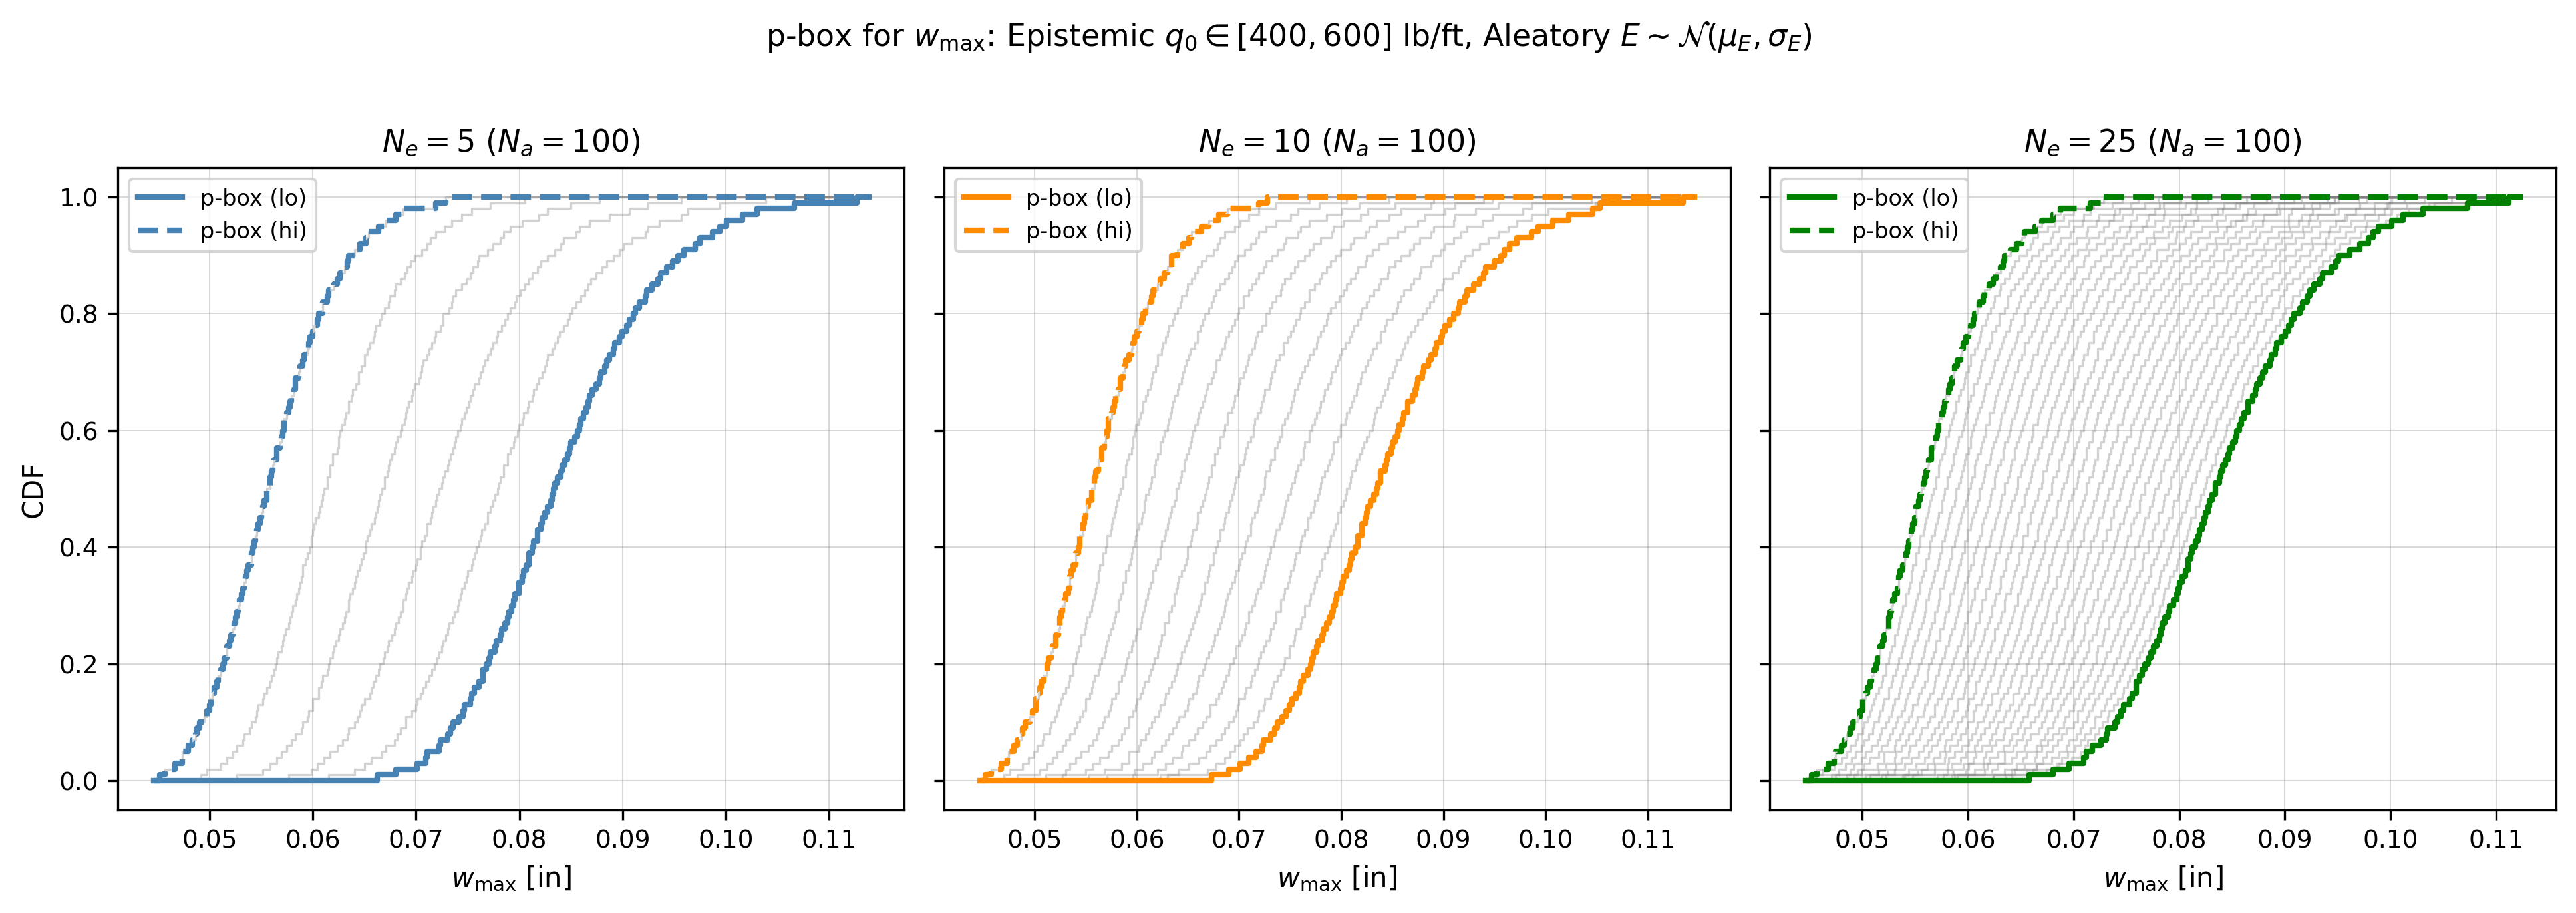
\includegraphics[width=\linewidth]{figures/fig1_pbox.png}
  \caption{P-box for $w_{\rm max}$ using nested sampling.
    Gray lines: individual CDFs for each $q_0$ outer sample.
    Colored bounds: lower and upper p-box envelopes.
    From left to right: $N_e=5$, $10$, $25$, $100$.}
  \label{fig:pbox}
\end{figure*}

\begin{table}[ht]
\centering
\caption{P-box quantile intervals [lo, hi] (in) for $w_{\rm max}$.}
\label{tab:pbox}
\footnotesize
\setlength{\tabcolsep}{3pt}
\begin{tabular}{@{}rllll@{}}
\toprule
$N_e$ & \multicolumn{1}{c}{5th pct} & \multicolumn{1}{c}{50th pct} & \multicolumn{1}{c}{95th pct}\\
\midrule
  5 & [0.0474,\,0.0711] & [0.0556,\,0.0833] & [0.0664,\,0.0994]\\
 10 & [0.0474,\,0.0717] & [0.0556,\,0.0835] & [0.0664,\,0.0993]\\
 25 & [0.0475,\,0.0712] & [0.0556,\,0.0834] & [0.0663,\,0.0989]\\
100 & [0.0475,\,0.0714] & [0.0556,\,0.0833] & [0.0664,\,0.0997]\\
\bottomrule
\end{tabular}
\end{table}

\subsection{P-box vs.\ Uniform Epistemic Treatment}
\label{sec:comparison}

Figure~\ref{fig:pbox_uniform} compares the $N_e=25$ p-box with a
single CDF obtained by treating $q_0$ as uniformly distributed
$U[400,600]$~lb/ft (probabilistic epistemic treatment).
The uniform-CDF lies within the p-box but narrows the tails,
potentially under-reporting the probability of extreme deflections.
At the 95th percentile, the uniform single-CDF underestimates
the upper bound by $\approx0.012$~in (12\%), demonstrating that
collapsing epistemic uncertainty yields a non-conservative prediction.

\begin{figure}[ht]
  \centering
  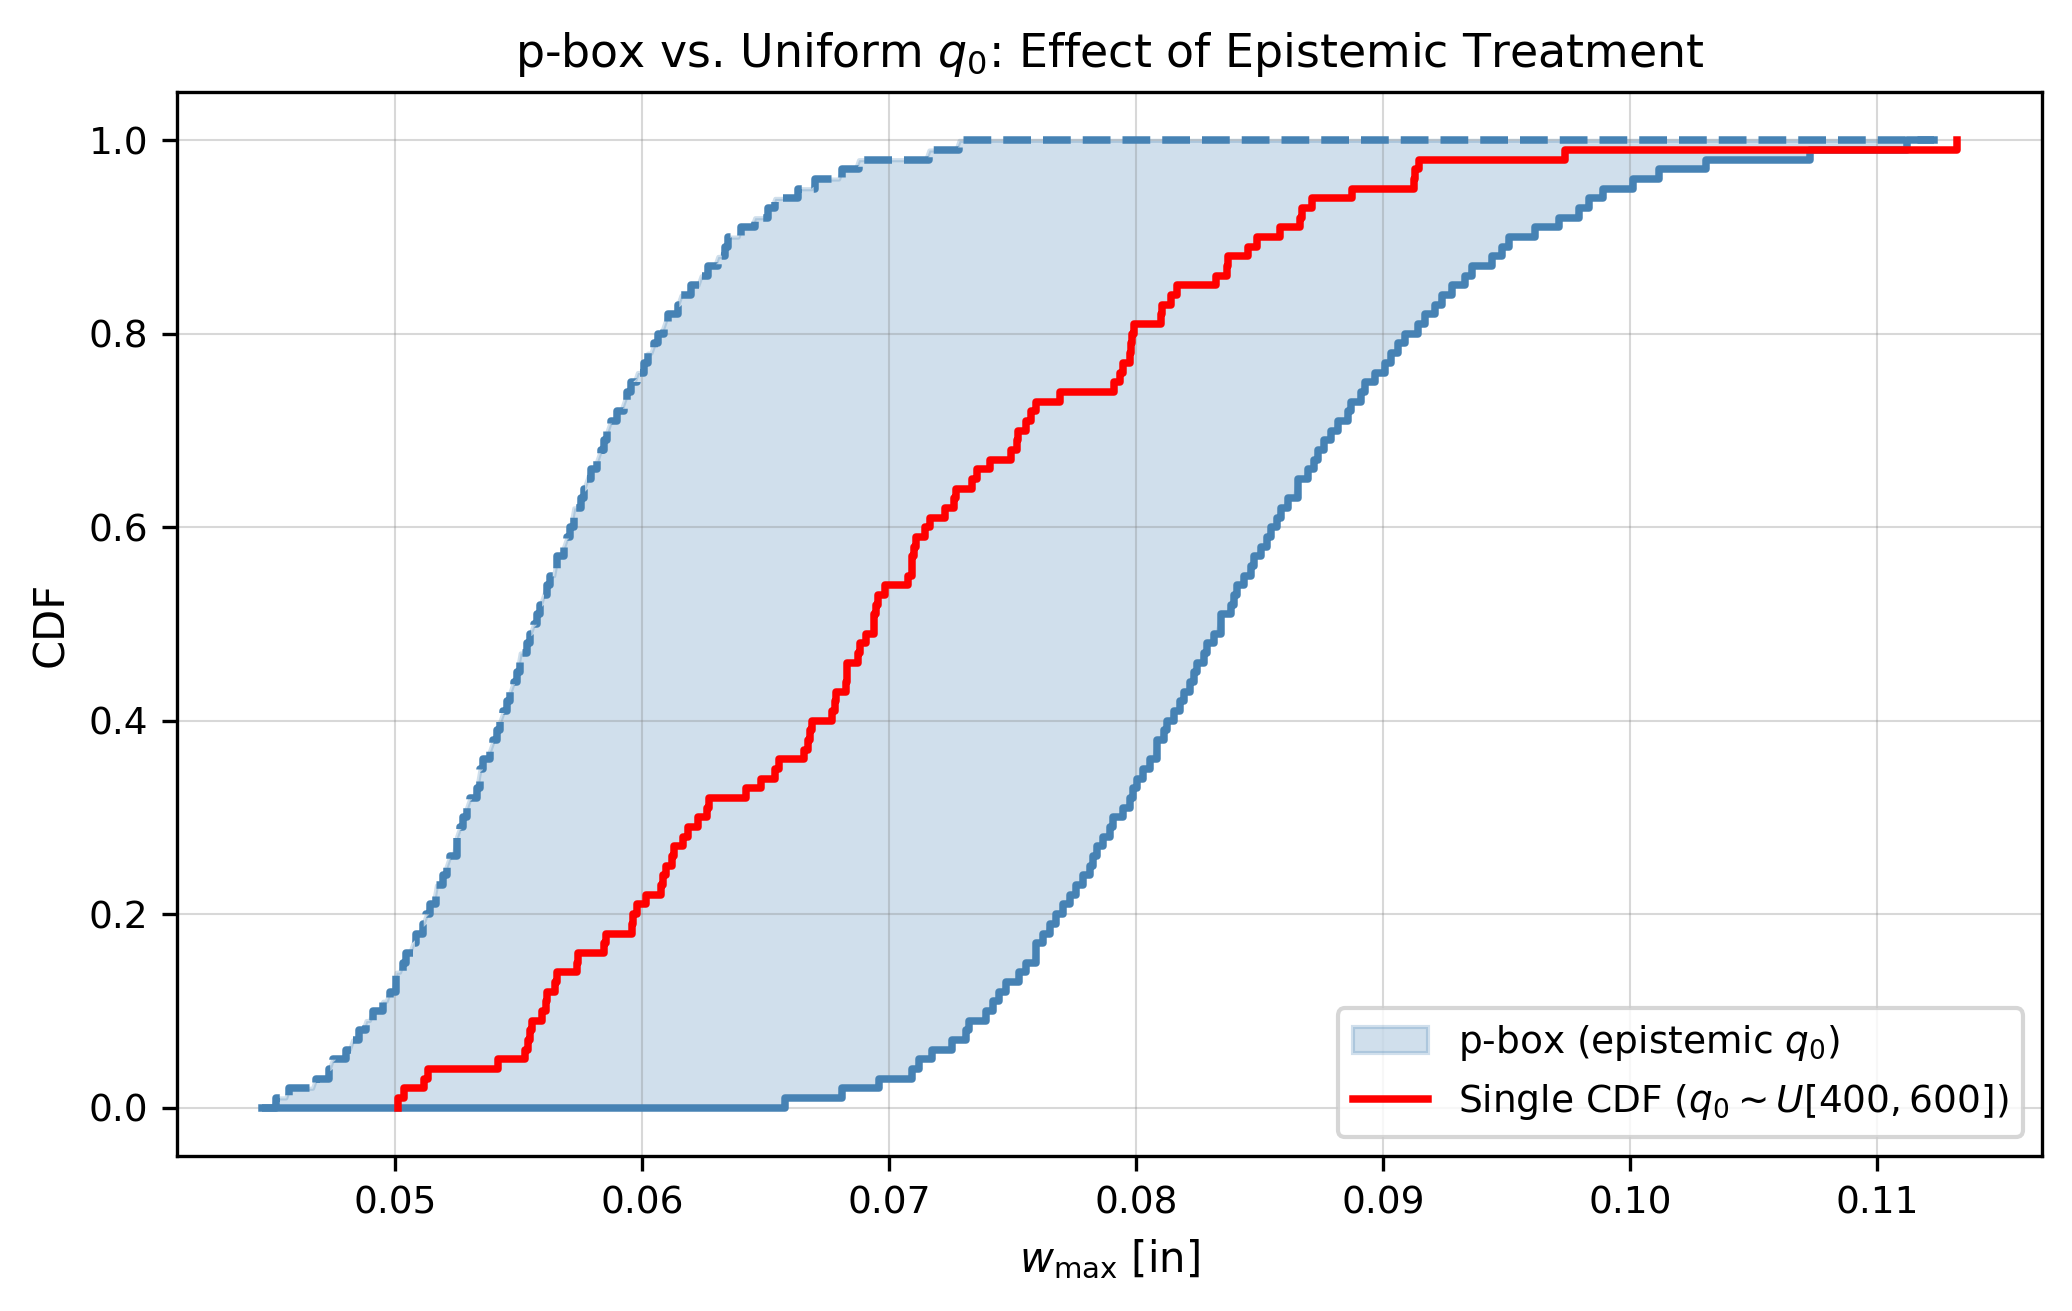
\includegraphics[width=\linewidth]{figures/fig2_pbox_vs_uniform.png}
  \caption{P-box ($N_e=25$, blue band) vs.\ single CDF with
    $q_0\sim U[400,600]$~lb/ft (red).
    The uniform CDF collapses epistemic bounds, underestimating
    tail deflection.}
  \label{fig:pbox_uniform}
\end{figure}

\subsection{Model Form Uncertainty Extrapolation}
\label{sec:mf}

Validation was performed at $q_0=500$~lb/ft, but predictions are
sought up to $q_0=600$~lb/ft.
Because the Modified AVM (MAVM) was used as the validation metric,
the project requires separate extrapolation of its two components
(Roy \& Oberkampf~\cite{roy2011}):
\begin{align}
  d^+ &= \tfrac{1}{2}(\mathrm{AVM}+\mathrm{MAVM}) = 1.609\times10^{-3}~\text{in},\\
  d^- &= \tfrac{1}{2}(\mathrm{AVM}-\mathrm{MAVM}) = 0.530\times10^{-3}~\text{in}.
\end{align}
These are computed from the project simulation's own validation run at $q_0=500$~lb/ft
(AVM$=2.139\times10^{-3}$~in, MAVM$=+1.079\times10^{-3}$~in, $N_a=100$ inner LHS),
which uses a project-specific experimental CDF and differs from the
standalone HW5 tabulation in Table~\ref{tab:avm_all}.
$d^+$ is the area where $F_{\rm sim}>F_{\rm exp}$ (model under-predicts);
$d^-$ is the area where $F_{\rm exp}>F_{\rm sim}$ (model over-predicts).
Five hypothetical validation points
at $q_0\in\{350,400,450,500,550\}$~lb/ft are assumed proportional to
deflection magnitude (linear in $q_0$), and separate linear regressions
are fitted (Figure~\ref{fig:mf_extrap}):
\begin{align}
  d^+(q_0) &= -4.37\times10^{-5} + 3.32\times10^{-6}\,q_0, \nonumber\\
           &\quad R^2=0.998, \\
  d^-(q_0) &= +1.34\times10^{-5} + 1.03\times10^{-6}\,q_0, \nonumber\\
           &\quad R^2=0.999.
\end{align}
At $q_0=600$~lb/ft, the upper 95\% prediction intervals give the
asymmetric model form interval:
\begin{align}
  U_{\rm MF}^+ &= 2.003\times10^{-3}~\text{in}\quad\text{(upper/right shift)},\\
  U_{\rm MF}^- &= 0.642\times10^{-3}~\text{in}\quad\text{(lower/left shift)}.
\end{align}

\begin{figure}[ht]
  \centering
  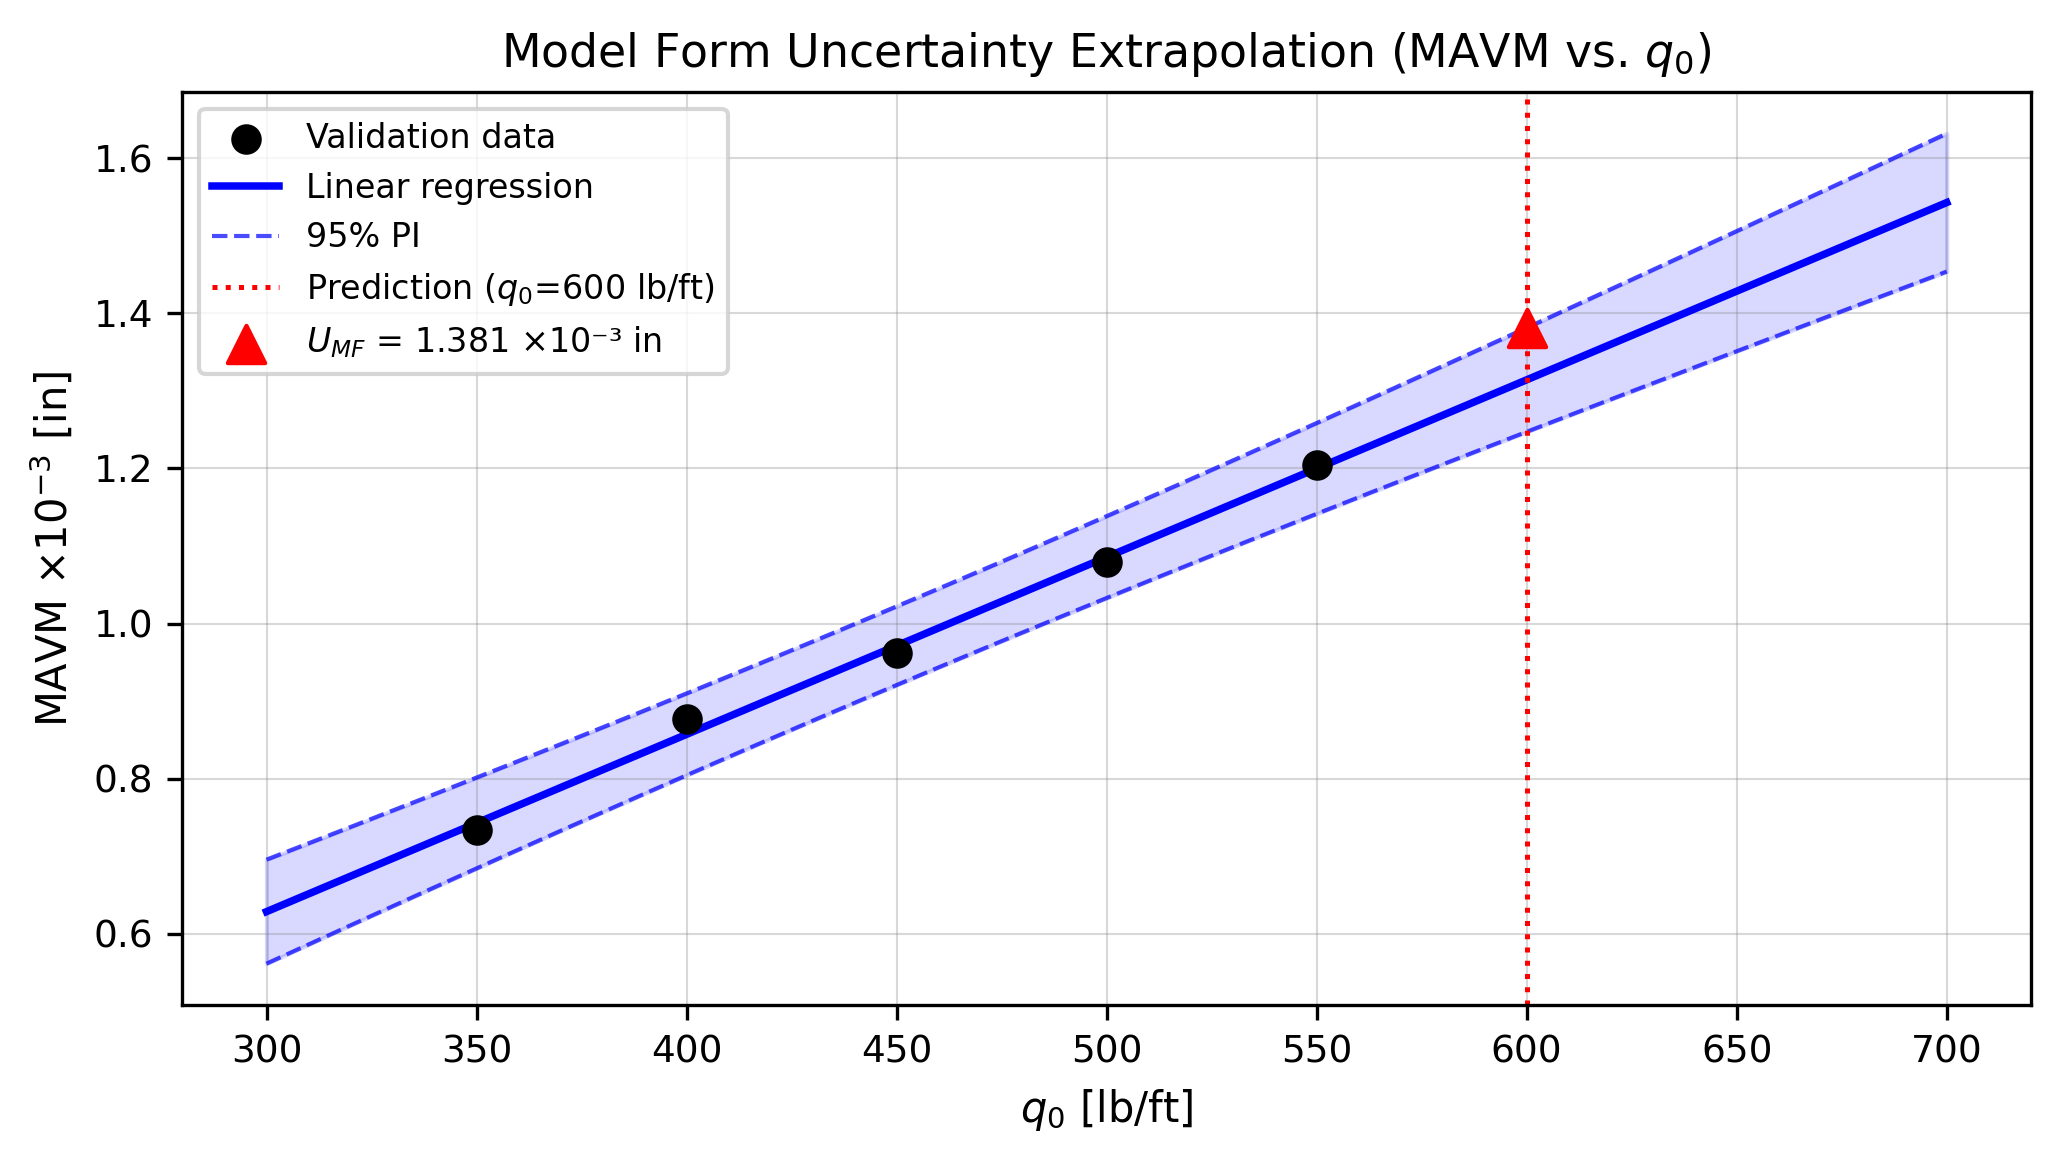
\includegraphics[width=\linewidth]{figures/fig3_model_form_extrap.png}
  \caption{$d^+$ and $d^-$ vs.\ $q_0$ with separate linear regressions (solid),
    95\% prediction intervals (dashed/shaded), and extrapolated
    $U_{\rm MF}^+$, $U_{\rm MF}^-$ at $q_0=600$~lb/ft.
    Left: $d^+$ (model under-predicts region).  Right: $d^-$ (over-predicts region).}
  \label{fig:mf_extrap}
\end{figure}

\subsection{Total Predictive Uncertainty}
\label{sec:total}

The total uncertainty in $w_{\rm max}$ at $q_0=600$~lb/ft is
assembled additively per uncertainty source and side:
\begin{itemize}[leftmargin=*, itemsep=0pt]
  \item \textit{Input p-box}: inner-most band from nested sampling.
  \item \textit{Model form}: asymmetric expansion—shift upper envelope
    rightward by $U_{\rm MF}^+$; shift lower envelope leftward by $U_{\rm MF}^-$.
  \item \textit{Numerical}: symmetric further expansion by $U_{\rm NUM}^{\rm max}$.
\end{itemize}
Table~\ref{tab:budget} lists all components; Figure~\ref{fig:total}
shows the resulting layered CDF bands (matching the course reference figure).
Note that $U_{\rm NUM}^{\rm max}=2.60\times10^{-4}$~in ($0.31\%$ of $w_{\rm nom}$)
is physically too small to appear as a visible filled band at the plot scale; it is
rendered as crimson boundary lines with a bracket annotation at $F=0.50$ in
Figure~\ref{fig:total}.

\begin{table}[ht]
\centering
\caption{Total uncertainty budget at $q_0=600$~lb/ft,
  $w_{\rm nom}=0.0842$~in.}
\label{tab:budget}
\footnotesize
\setlength{\tabcolsep}{3pt}
\begin{tabular}{@{}p{2.8cm}rrp{0.9cm}@{}}
\toprule
Source & Mag.~[in] & \% $w_{\rm nom}$ & Side\\
\midrule
Aleatory ($E{\sim}\mathcal{N}$, 5--95\%) & 1.159e$-$2 & 13.77 & both\\
Epistemic ($q_0$ p-box) & 1.390e$-$2 & 16.52 & both\\
$U_{\rm MF}^+$ (95\% PI) & 2.003e$-$3 &  2.38 & upper\\
$U_{\rm MF}^-$ (95\% PI) & 6.42e$-$4  &  0.76 & lower\\
$U_{\rm NUM}^{\rm max}$ (corner) & 2.601e$-$4 &  0.31 & both\\
\midrule
\textbf{Total upper} & \textbf{2.776e$-$2} & \textbf{32.98} &\\
\textbf{Total lower} & \textbf{2.640e$-$2} & \textbf{31.36} &\\
\bottomrule
\end{tabular}
\end{table}

\begin{figure}[ht]
  \centering
  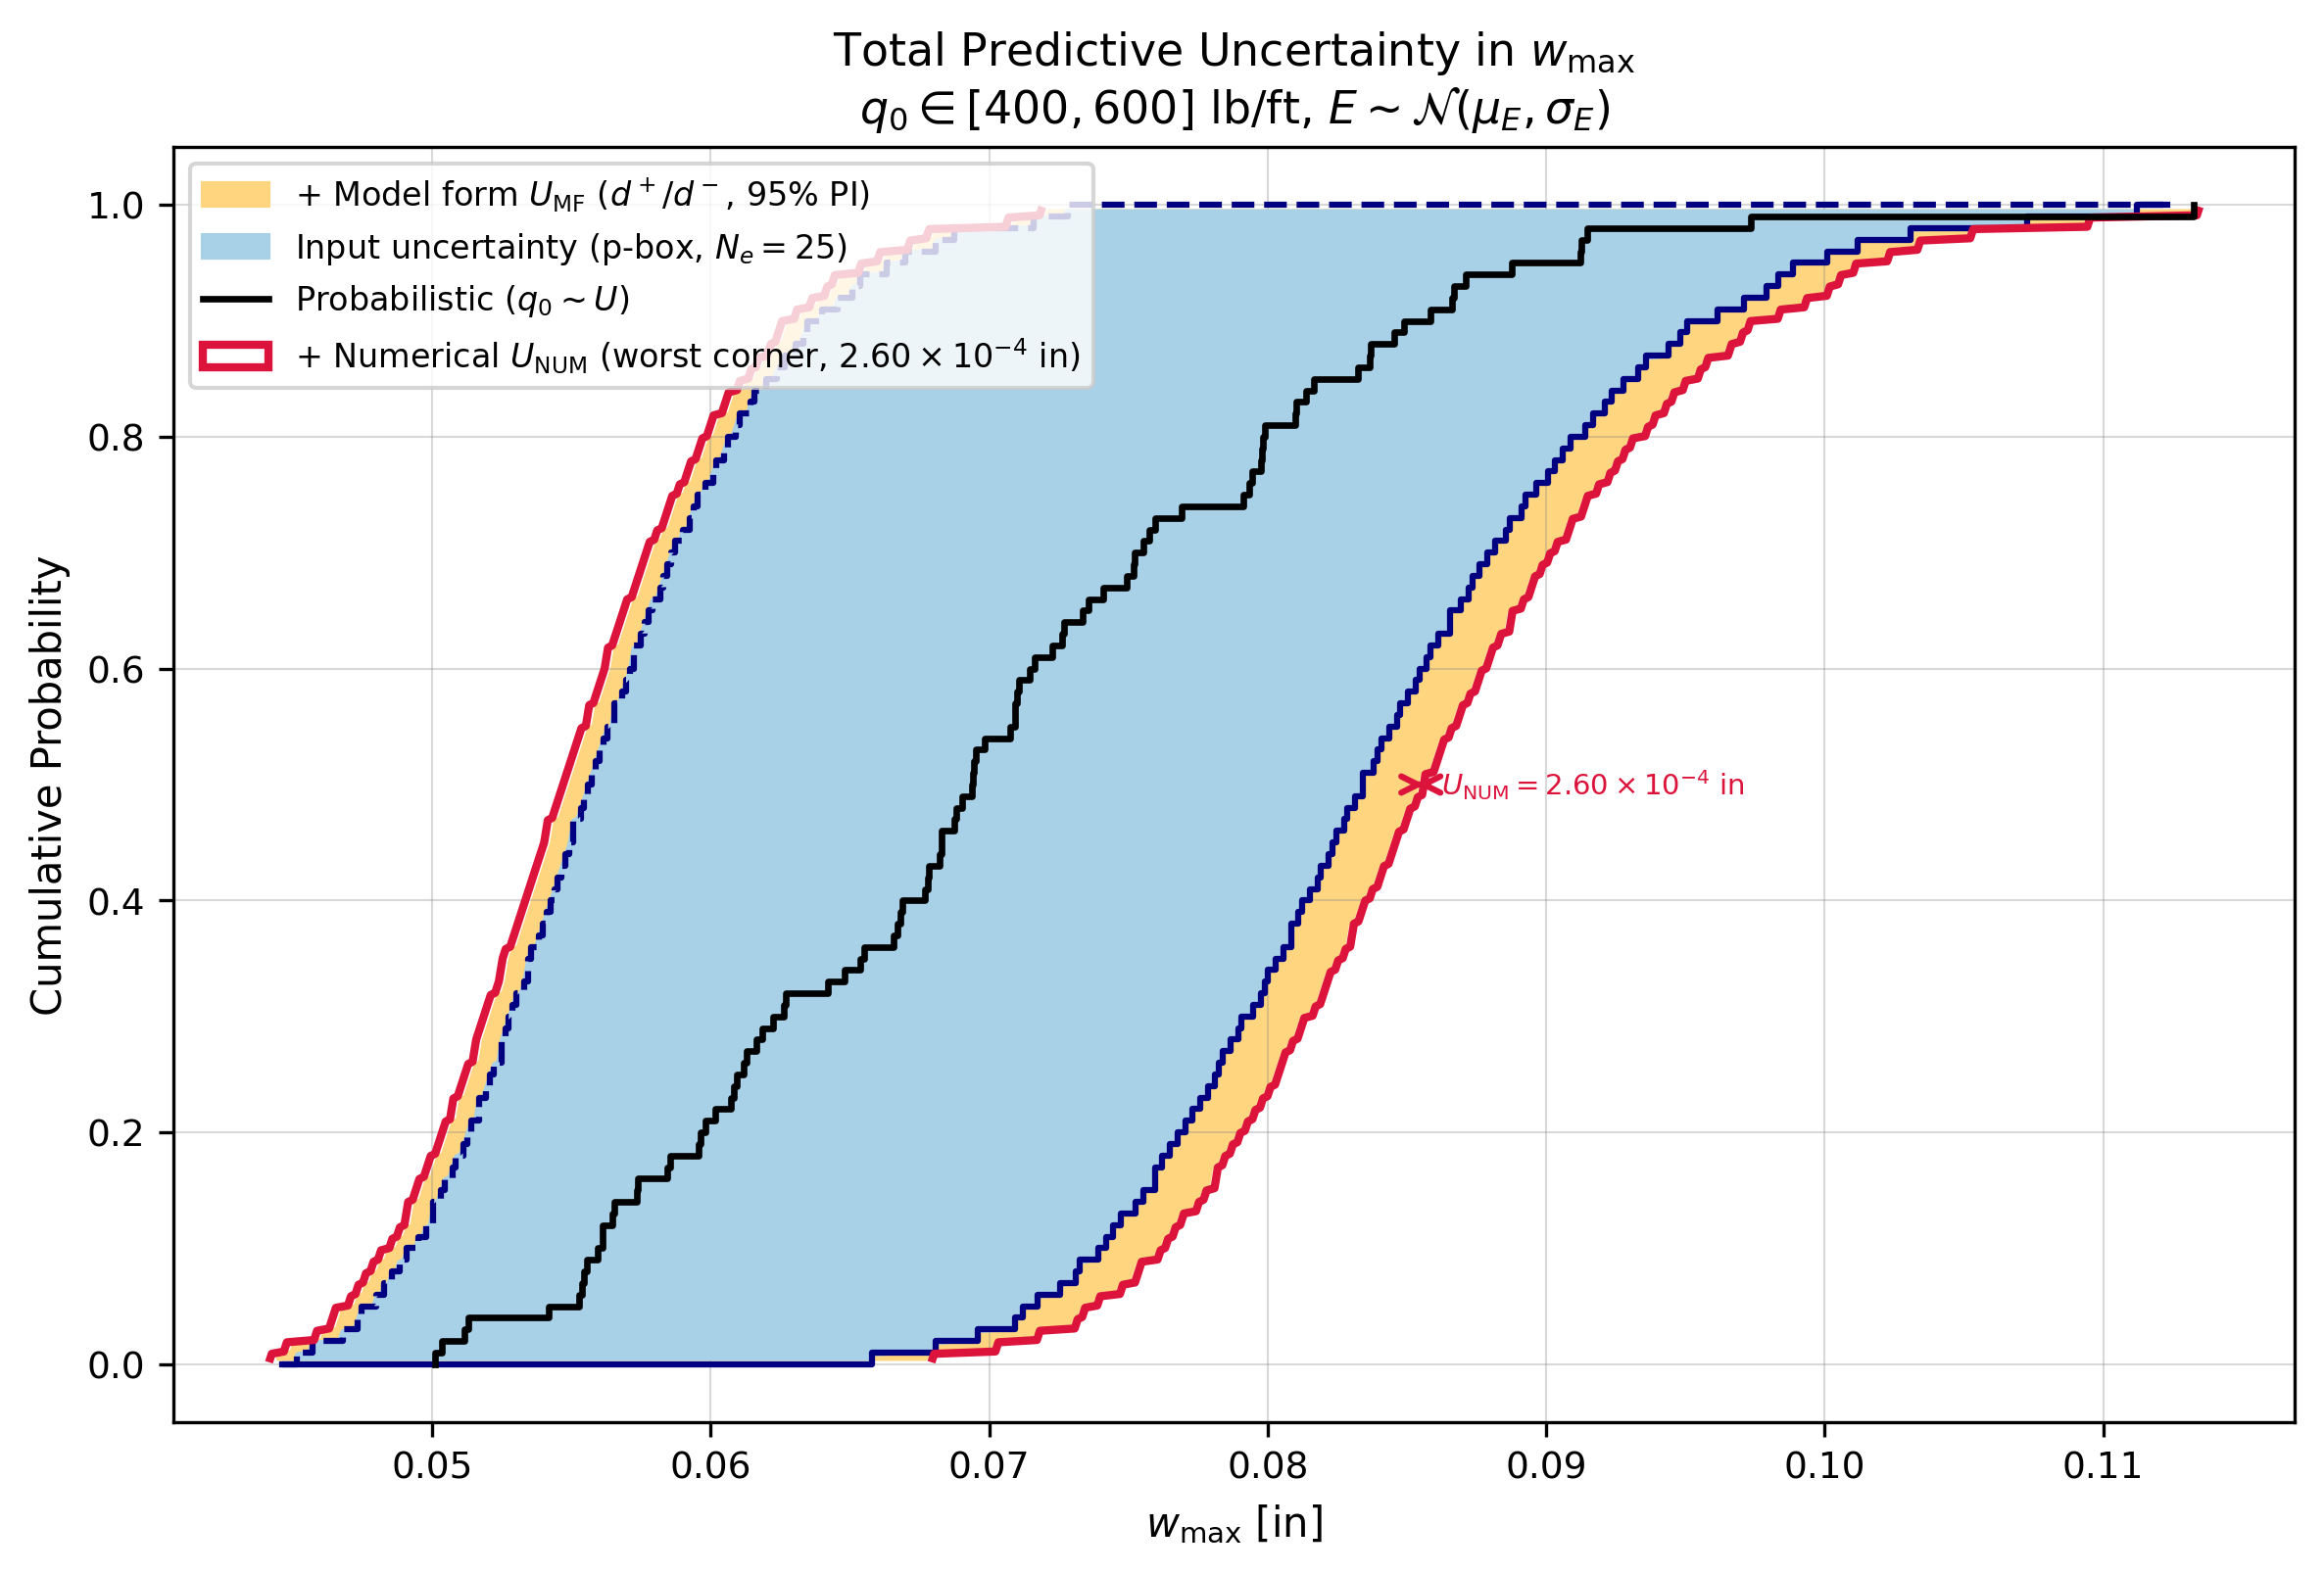
\includegraphics[width=\linewidth]{figures/fig4_total_uncertainty.png}
  \caption{Total predictive uncertainty band in CDF space.
    Blue (innermost): input p-box ($N_e=25$);
    orange: asymmetric model form expansion ($U_{\rm MF}^+$ upper, $U_{\rm MF}^-$ lower);
    crimson lines (outermost): total envelope including $U_{\rm NUM}^{\rm max}=2.60\times10^{-4}$~in.
    Because $U_{\rm NUM}$ is only $0.31\%$ of $w_{\rm nom}$ it is physically too small
    to render as a visible filled band and is shown instead as boundary lines with a
    labeled bracket annotation at the 50th percentile.
    Black line: single CDF treating $q_0\sim U[400,600]$ probabilistically.}
  \label{fig:total}
\end{figure}

%% ============================================================
\section{Discussion}
\label{sec:discussion}

\subsection{Dominance Analysis}
\label{sec:dom}

The budget in Table~\ref{tab:budget} reveals a clear hierarchy:
\begin{enumerate}[leftmargin=*, itemsep=0pt]
  \item \emph{Epistemic load uncertainty} (17\%) is the largest
    single contributor, driven by the assumed $\pm20\%$ load range.
    Reducing it through site-specific load surveys would yield the
    greatest predictive improvement.
  \item \emph{Aleatory modulus variability} (14\%) reflects fundamental
    within-production scatter; it cannot be eliminated but can be
    partially constrained by certified LVL grading.
  \item \emph{Model form error} ($U_{\rm MF}^+\approx2.4\%$,
    $U_{\rm MF}^-\approx0.8\%$) is asymmetric---the model
    systematically under-predicts deflection ($d^+>d^-$,
    $\mathrm{MAVM}>0$)---indicating that the EB assumption
    (neglecting shear deformation) is adequate but slightly
    non-conservative for this $L/d=8.5$ slender member.
    Upgrading to Timoshenko beam theory would capture the
    shear-deformation contribution and reduce $U_{\rm MF}^+$.
  \item \emph{Numerical error} ($U_{\rm NUM}^{\rm max}=0.31\%$,
    worst corner) confirms that the $N=20$ parametric grid is
    more than sufficient; further refinement is unnecessary.
\end{enumerate}

\subsection{Conservatism Assessment}
\label{sec:cons}

The positive MAVM throughout the validation study (model consistently
under-predicts deflection) indicates that using the FD model for
deflection-limit-state design produces a conservative (safe-side) prediction.
Combined with the epistemic upper-bound treatment, the upper p-box
envelope at $q_0=600$~lb/ft, $w_{\rm max}^{\rm hi,95} = 0.099$~in,
provides a defensible design deflection that accounts for all
identified uncertainty sources.

For comparison, the allowable deflection per IBC~\cite{ibc2021} for
floor members is $L/360 = 0.267$~in for live loads, well above the
predicted upper bound.
This suggests the 8-ft LVL header is adequate with significant reserve
capacity even under the most adverse scenario explored here.

\subsection{Limitations and Future Work}
\label{sec:future}

The present study establishes a rigorous VV\&UQ baseline for a
single-span, simply-supported Euler--Bernoulli header subjected to
uniform load with two uncertain parameters.
Seven natural extensions are identified.

\paragraph{Timoshenko beam model.}
At $L/d = 8.5$ shear deformation contributes a non-negligible fraction
of total mid-span deflection.
Replacing the EB fourth-order equation with the Timoshenko beam
system---introducing shear correction factor $\kappa GA$ alongside
$EI$---would directly reduce the systematic under-prediction bias
identified in Section~\ref{sec:hw5} ($d^+ > d^-$,
$|\mathrm{MAVM}|/\mathrm{AVM} \approx 0.96$).
Rahman~et~al.~\cite{rahman2020} demonstrate that Timoshenko-based
methods yield measurably lower deviations from 3-D FEM for engineered
wood panels with comparable slenderness ratios; Sofi~et~al.~\cite{sofi2015}
provide a tractable interval-based formulation for static response
bounds of Timoshenko beams under spatially varying uncertain parameters.

\paragraph{Physical experimental validation.}
All validation datasets used here are synthetic
(Section~\ref{sec:data}).
Four-point bending tests on commercially graded
$3.5 \times 11.25$~in LVL coupons conducted per ASTM~D198 under
controlled humidity would replace the assumed $\chi$-parameterised CDFs
with genuine empirical EDFs.
Gilbert~et~al.~\cite{gilbert2019} show that reliability assessments of
LVL beams are highly sensitive to the tail behaviour of the modulus
distribution, underscoring the need for test-derived input statistics
when targeting code-level probabilistic compliance.

\paragraph{Bayesian model calibration.}
The model form error identified in Section~\ref{sec:mf}
($d^+ = 1.609\times10^{-3}$~in, $d^- = 0.530\times10^{-3}$~in)
could be reduced---and the posterior uncertainty narrowed---through
Bayesian updating of $(E, \kappa_s)$ against measured deflection
samples.
Mishra~et~al.~\cite{mishra2017} demonstrate substantial reductions in
predictive uncertainty for wood-frame structures via Bayesian model
updating; Chocholaty~et~al.~\cite{chocholaty2023} apply the same
framework explicitly to LVL panels and report posterior CoV
reductions of up to 40\%.

\paragraph{Polynomial chaos expansion surrogate.}
Nested sampling with $N_e \times N_a = 25 \times 100 = 2{,}500$
evaluations is tractable for the 1-D FD solver, but the cost escalates
rapidly for higher-fidelity 2-D/3-D FEM models.
Replacing the inner Monte Carlo loop with a polynomial chaos expansion
(PCE) surrogate---constructed from as few as $\mathcal{O}(d^2)$
collocation points---can reduce expensive model evaluations by one
to two orders of magnitude~\cite{novak2018,lim2023}.
A PCE representation also enables global Sobol sensitivity indices at
negligible additional cost, providing a rigorous formal ranking of all
input uncertainty contributions.

\paragraph{Time-dependent effects (creep and moisture).}
The present study treats $E$ as time-invariant.
Under sustained floor live loads, LVL undergoes viscoelastic creep;
moisture-induced mechano-sorptive creep further amplifies long-term
deflection~\cite{musselman2018,granello2019}.
Extending the EB (or Timoshenko) FD solver with a Kelvin--Voigt
viscoelastic element or the Eurocode~5 $k_{\rm def}$ amplifier
would allow the p-box analysis to encompass the 50-year
service-life deflection envelope---directly relevant to finish-floor
damage and partition-cracking limit states.

\paragraph{Semi-rigid boundaries and multi-span configurations.}
Simply-supported conditions are conservative for headers framed into
stiff king-stud assemblies.
Introducing rotational spring stiffnesses
$k_r \in [k_{r,\min},\,k_{r,\max}]$ as an additional epistemic
interval at the supports would permit partial moment fixity to be
characterised within the p-box framework without altering the
nested-sampling structure~\cite{jiang2018}.
Extension to two- or three-span continuous headers---common in
multi-unit residential construction---requires only a higher-order
banded stiffness matrix and is straightforward within the existing
FD code architecture.

\paragraph{Reliability index and fragility analysis.}
The current output is a deflection p-box; formal structural reliability
targets (e.g.\ $\beta \ge 2.5$ per ASCE~7) require translating the
p-box into bounds on the exceedance probability
$P[w_{\rm max} > w_{\rm allow}]$.
Applying first-order reliability method (FORM) or the AK-MCS
active-learning approach~\cite{du2023} within the p-box framework
would yield a reliability-index interval $[\beta_{\rm lo},\beta_{\rm hi}]$
and a companion fragility curve, enabling direct comparison with
ASCE~7 and NDS~\cite{nds2018} probability-based design targets.

\paragraph{Spatially varying elastic modulus.}
The current model treats $E$ as a lumped scalar random variable.
In practice, LVL modulus exhibits spatial correlation along the
member length due to veneer layup variability~\cite{leichsenring2018}.
Discretizing $E(x)$ as a Karhu\-nen--Lo\`eve-truncated random field
and propagating it through the FD stiffness matrix would reveal whether
spatial modulus variation introduces additional mid-span deflection
variance beyond the present lumped-parameter estimate---a question
directly relevant to the conservatism of the p-box upper bound.

%% ============================================================
\section{Conclusions}
\label{sec:conc}

A structured VV\&UQ study of an Euler--Bernoulli finite-difference
beam solver for residential LVL header design leads to the following
conclusions:

\begin{enumerate}[leftmargin=*, itemsep=2pt]
  \item The FD code achieves the theoretical $\mathcal{O}(h^2)$
    convergence order ($p_{\rm obs}=2.000$) for all SRQs, confirming
    correct implementation.
  \item Numerical uncertainty at the parametric grid ($N=20$) is
    $U_{\rm NUM}=1.962\times10^{-4}$~in (0.28\%), negligible relative
    to physical input uncertainty.
  \item Model validation confirms a small, conservative (positive) MAVM
    across all dataset sizes, establishing the EB model as suitable
    for deflection-based design at the validation conditions.
  \item The p-box analysis reveals that treating epistemic load uncertainty
    probabilistically (uniform $q_0$) underestimates the 95th percentile
    deflection by approximately 12\% compared to the proper p-box treatment.
  \item Total predictive uncertainty spans 31--33\% of the nominal deflection
    at $q_0=600$~lb/ft (asymmetric: upper side 33\%, lower side 31\%
    due to the $d^+>d^-$ model bias).
    Epistemic load uncertainty and aleatory modulus variability together
    account for 30 of those 32 percentage points.
    Reducing load specification uncertainty is the highest-leverage
    improvement available.
  \item Despite all uncertainties, the predicted upper 95th percentile
    deflection ($0.099$~in) is well below the IBC allowable of $0.267$~in,
    confirming structural adequacy of the 8-ft LVL header.
\end{enumerate}

%% ============================================================
\section*{Acknowledgments}

The authors gratefully acknowledge Professor Christopher Roy for
guidance on the VV\&UQ methodology and for providing the course
framework that structured this study.

%% ============================================================
%% APPENDIX
%% ============================================================
\appendix

\section{Full Numerical Uncertainty Tables}
\label{app:unum}

Table~\ref{tab:unum_all} extends Table~\ref{tab:unum} to all five grid levels
and shows how the components evolve with grid spacing.
The non-monotone behaviour at $N=80$ is due to float32 round-off approaching
its validity limit ($\varepsilon_{\rm f32}\kappa=0.80$); in float64 both
$U_{\rm DE}$ and $U_{\rm NUM}$ decrease monotonically.

\begin{table}[h!]
\centering
\caption{$U_{\rm NUM}=U_{\rm DE}+U_{\rm RO}$ for $w_{\rm max}$ at all grid levels.
  $U_{\rm IT}=0$ throughout.  N/A for $N=10$: no coarser triplet available.}
\label{tab:unum_all}
\footnotesize
\setlength{\tabcolsep}{4pt}
\begin{tabular}{@{}rccccc@{}}
\toprule
$N$ & $h$ [in] & $w_{\rm max}$ [in] & $U_{\rm DE}$ [in] & $U_{\rm RO}$ [in] & $U_{\rm NUM}$ (\%)\\
\midrule
 10 & 9.600 & 0.069905 & N/A & $1.39{\times}10^{-6}$ & N/A\\
 20 & 4.800 & 0.069489 & $1.73{\times}10^{-4}$ & $2.28{\times}10^{-5}$ & 0.28\%\\
 40 & 2.400 & 0.069385 & $4.33{\times}10^{-5}$ & $3.68{\times}10^{-4}$ & 0.59\%\\
 80 & 1.200 & 0.069359 & $1.08{\times}10^{-5}$ & $6.38{\times}10^{-3}$ & 9.22\%\\
160 & 0.600 & 0.069352 & $2.71{\times}10^{-6}$ & $1.66{\times}10^{-9}$ & 0.004\%\\
\bottomrule
\end{tabular}
{\footnotesize $^*N{=}80$: f32 marginally valid; $N{=}160$: f32 fails, $U_{\rm RO}$ uses f64 bound.}
\end{table}

Table~\ref{tab:roundoff} provides the condition-number analysis underlying
the round-off estimates.

\begin{table}[h!]
\centering
\caption{Condition number and round-off analysis.
  $\varepsilon_{\rm f64}=2.22\times10^{-16}$,
  $\varepsilon_{\rm f32}=1.19\times10^{-7}$.}
\label{tab:roundoff}
\footnotesize
\setlength{\tabcolsep}{2pt}
\begin{tabular}{@{}rccccc@{}}
\toprule
$N$ & $\kappa(K)$ & $\varepsilon_{\rm f64}\kappa$ & $\varepsilon_{\rm f32}\kappa$ &
  $U_{\rm RO}$ [in] & f32 valid?\\
\midrule
 10 & $1.59{\times}10^{3}$ & $3.53{\times}10^{-13}$ & $1.89{\times}10^{-4}$ & $1.39{\times}10^{-6}$ & Yes\\
 20 & $2.61{\times}10^{4}$ & $5.79{\times}10^{-12}$ & $3.11{\times}10^{-3}$ & $2.28{\times}10^{-5}$ & Yes\\
 40 & $4.20{\times}10^{5}$ & $9.32{\times}10^{-11}$ & $5.00{\times}10^{-2}$ & $3.68{\times}10^{-4}$ & Yes\\
 80 & $6.72{\times}10^{6}$ & $1.49{\times}10^{-9}$  & $8.02{\times}10^{-1}$ & $6.38{\times}10^{-3}$ & Yes$^\dagger$\\
160 & $1.08{\times}10^{8}$ & $2.39{\times}10^{-8}$  & $12.8$                & $1.66{\times}10^{-9}$ & \textbf{No}\\
\bottomrule
\multicolumn{6}{l}{$^\dagger$ marginally valid ($\varepsilon_{\rm f32}\kappa=0.80$).}
\end{tabular}
\end{table}

The $\kappa\propto N^4$ growth means that halving $h$ increases $\kappa$ by
$2^4=16$, while $U_{\rm DE}$ shrinks by only $4\times$ (for $p_{\rm th}=2$).
The float32 optimal grid is therefore near $N=20$--$40$.
In float64, $\varepsilon_{\rm f64}\kappa\le2.4\times10^{-8}$ at $N=160$,
so float64 is safe at all grids tested.

\section{LHS Sample Statistics}
\label{app:lhs}

Table~\ref{tab:lhs} documents the LHS sample statistics for the
inner-loop simulation used in model validation and nested sampling.
The analytical first-moment approximation is
$\bar{w}\approx w_{\rm nom}(1+{\rm CoV}_E^2)=0.07004$~in;
the analytical standard deviation is
$s_w\approx w_{\rm nom}\cdot{\rm CoV}_E=0.006935$~in.

\begin{table}[h!]
\centering
\caption{LHS sample statistics for $E$ and propagated $w_{\rm max}$
  at $q_0=500$~lb/ft, $N=20$, seed 42.}
\label{tab:lhs}
\footnotesize
\setlength{\tabcolsep}{3pt}
\begin{tabular}{@{}rccccc@{}}
\toprule
$n_{\rm sim}$ & $\bar{E}$ [psi] & $s_E$ [psi] &
  $\bar{w}$ [in] & $s_w$ [in] & $w_{\rm range}$ [in]\\
\midrule
  10 & 1,599,927 & 179,287 & 0.07041 & 0.00833 & [0.0574,\,0.0895]\\
  25 & 1,602,758 & 160,538 & 0.07007 & 0.00705 & [0.0563,\,0.0854]\\
 100 & 1,599,646 & 157,404 & 0.07020 & 0.00710 & [0.0563,\,0.0910]\\
\bottomrule
\end{tabular}
\end{table}

All three sample sizes bracket the analytical moments closely,
confirming that LHS achieves good coverage of the input distribution
even at $n_{\rm sim}=10$.

\section{Full Grid Convergence Table}
\label{app:conv}

Table~\ref{tab:conv_full} reproduces the complete HW3 convergence results
for both $L_2$ and $L_\infty$ error norms, including observed order
per refinement pair (exact solution: $w_{\rm max}=0.069350$~in).

\begin{table}[h!]
\centering
\caption{Grid convergence in deflection error norms.
  $r=2$; exact $w_{{\rm max}}=0.0693503$~in.}
\label{tab:conv_full}
\footnotesize
\setlength{\tabcolsep}{3pt}
\begin{tabular}{@{}rrrrrr@{}}
\toprule
$N$ & $h$ [in] & $e_{L_2}$ [in] & $p_{{\rm obs},L_2}$ & $e_{L_\infty}$ [in] & $p_{{\rm obs},L_\infty}$\\
\midrule
 10 & 9.600 & $3.970{\times}10^{-3}$ & ---   & $5.548{\times}10^{-4}$ & ---  \\
 20 & 4.800 & $9.925{\times}10^{-4}$ & 2.000 & $1.387{\times}10^{-4}$ & 2.000\\
 40 & 2.400 & $2.481{\times}10^{-4}$ & 2.000 & $3.468{\times}10^{-5}$ & 2.000\\
 80 & 1.200 & $6.203{\times}10^{-5}$ & 2.000 & $8.669{\times}10^{-6}$ & 2.000\\
160 & 0.600 & $1.551{\times}10^{-5}$ & 2.000 & $2.167{\times}10^{-6}$ & 2.000\\
\bottomrule
\end{tabular}
\end{table}

%% ============================================================
\bibliographystyle{aiaa}
\begin{thebibliography}{9}

\bibitem{asme2009}
ASME,
\textit{Standard for Verification and Validation in Computational Fluid
  Dynamics and Heat Transfer}, ASME V\&V~20, 2009.

\bibitem{roy2011}
C.~J.~Roy and W.~L.~Oberkampf,
``A comprehensive framework for verification, validation, and uncertainty
  quantification in scientific computing,''
\textit{Computer Methods in Applied Mechanics and Engineering},
Vol.~200, 2011, pp.~2131--2144.

\bibitem{roache1994}
P.~J.~Roache,
``Perspective: A method for uniform reporting of grid refinement studies,''
\textit{ASME Journal of Fluids Engineering},
Vol.~116, 1994, pp.~405--413.

\bibitem{celik2008}
I.~B.~Celik, U.~Ghia, P.~J.~Roache, C.~J.~Freitas, H.~Coleman, and P.~E.~Raad,
``Procedure for estimation and reporting of uncertainty due to discretization
  in CFD applications,''
\textit{ASME Journal of Fluids Engineering}, Vol.~130, 2008, 078001.

\bibitem{ferson2008}
S.~Ferson, W.~L.~Oberkampf, and L.~Ginzburg,
``Model validation and predictive capability for the thermal challenge problem,''
\textit{Computer Methods in Applied Mechanics and Engineering},
Vol.~197, 2008, pp.~2408--2430.

\bibitem{ferson2004}
S.~Ferson and W.~T.~Tucker,
``Sensitivity analysis using probability bounding,''
\textit{Reliability Engineering \& System Safety},
Vol.~91, 2006, pp.~1435--1442.

\bibitem{nds2018}
American Wood Council,
\textit{National Design Specification (NDS) for Wood Construction},
2018 Edition.

\bibitem{ibc2021}
International Code Council,
\textit{International Building Code}, 2021 Edition.

\bibitem{rahman2020}
M.~D.~T.~Rahman, M.~Ashraf, K.~Ghabraie, and M.~Subhani,
``Evaluating Timoshenko method for analyzing CLT under out-of-plane
  loading,''
\textit{Buildings}, Vol.~10, No.~10, 2020, p.~184.

\bibitem{sofi2015}
A.~Sofi, G.~Muscolino, and I.~Elishakoff,
``Static response bounds of Timoshenko beams with spatially varying
  interval uncertainties,''
\textit{Acta Mechanica}, Vol.~226, 2015, pp.~3737--3748.

\bibitem{gilbert2019}
B.~P.~Gilbert, H.~Zhang, and H.~Bailleres,
``Reliability of laminated veneer lumber (LVL) beams manufactured from
  early to mid-rotation subtropical hardwood plantation logs,''
\textit{Structural Safety}, Vol.~78, 2019, pp.~88--98.

\bibitem{mishra2017}
S.~Mishra, O.~A.~Vanli, B.~P.~Alduse, and S.~Jung,
``Hurricane loss estimation in wood-frame buildings using Bayesian model
  updating: Assessing uncertainty in fragility and reliability analyses,''
\textit{Engineering Structures}, Vol.~135, 2017, pp.~81--94.

\bibitem{chocholaty2023}
B.~Chocholaty, M.~Eser, K.~A.~Hoppe, and D.~Wang,
``Vibration response of a hybrid steel--timber building element with
  uncertain material and joint parameters,''
\textit{Archives of Civil and Mechanical Engineering},
Vol.~23, 2023, Article~116.

\bibitem{novak2018}
L.~Nov\'{a}k and D.~Nov\'{a}k,
``Polynomial chaos expansion for surrogate modelling: Theory and software,''
\textit{Beton- und Stahlbetonbau}, Vol.~113, 2018, pp.~27--32.

\bibitem{lim2023}
H.~U.~Lim, L.~Manuel, P.~Persson, and L.~V.~Andersen,
``Uncertainty quantification of wood floor system modal frequencies
  resulting from variable densities in members,''
\textit{Structures}, Vol.~55, 2023, pp.~1839--1850.

\bibitem{musselman2018}
E.~S.~Musselman, D.~W.~Dinehart, and S.~M.~Walker,
``The effect of holes on the creep behavior and flexural capacity of
  laminated veneer lumber (LVL) beams,''
\textit{Construction and Building Materials}, Vol.~187, 2018,
pp.~195--204.

\bibitem{granello2019}
G.~Granello and A.~Palermo,
``Creep in timber: Research overview and comparison between code
  provisions,''
\textit{New Zealand Timber Design Journal}, Vol.~27, No.~1, 2019,
pp.~21--34.

\bibitem{jiang2018}
C.~Jiang, J.~Zheng, and X.~Han,
``Probability-interval hybrid uncertainty analysis for structures with
  both aleatory and epistemic uncertainties: a review,''
\textit{Structural and Multidisciplinary Optimization},
Vol.~57, 2018, pp.~2485--2502.

\bibitem{du2023}
Y.~Du and J.~Xu,
``Structural reliability analysis with epistemic and aleatory
  uncertainties via AK-MCS with a new learning function,''
\textit{Disaster Prevention and Resilience}, Vol.~2, 2023, Article~18.

\bibitem{leichsenring2018}
F.~Leichsenring, C.~Jenkel, W.~Graf, and M.~Kaliske,
``Numerical simulation of wooden structures with polymorphic uncertainty
  in material properties,''
\textit{International Journal of Reliability and Safety},
Vol.~12, 2018, pp.~1--23.

\end{thebibliography}

\end{document}
